\section{Experiment 1: Feature Extraction}
The python version CIFAR10 and CIFAR100 datasets are downloaded from the official website with pre-defined train and test sets. The train set were split into train and validation sets with the ratio 8:2 randomly. We got 40,000 train samples, 10,000 validation samples and 10,000 test samples for both datasets. In order to speed up the experiments, we started by extracting the image feature vectors with a single forward propagation before training the FC layers.

All trainable parameters of the two FC layers were initialised by the Xavier uniform method \cite{Glorot2010}. The training process was monitored by the validation accuracy. After each epoch, we reported the validation accuracy and kept a record of the model parameters which achieved the best validation accuracy so far. We scheduled two training stages to approach the optimal classification accuracy. First we performed 500 training epochs with step size 0.01 then decreased it to 0.001 for another 500 epochs.  After each training stage, the recorded parameters were loaded to prevent overfitting. The final held-out test set accuracy for CIFAR10 is 0.9258 and for CIFAR100 is 0.7444. Finally we compressed the extracted 4032-D feature vectors with the 128-D FC layer.

We further took a closer look at the compressed features by projecting them down to two dimensional vectors with t-SNE \cite{Maaten2008} and maintains the relative distance between samples. The plots are shown in Figure \ref{Fig.tsne}. Different colours represent different classes of samples. First of all, the network transformed the images into blobs where ideally samples from the same class should be closer to each other. This is true especially for CIFAR10. The quality of these compact blobs reflects the classification accuracy. Strays far from the cluster would be misclassified by the logistic regression layer thus lower the classification accuracy. Furthermore, the boundaries between different classes are not always clear. Blobs are close to each other near the boundary thus the classification accuracy is sensitive to slight variations of the boundary. The effect is more obvious if there are more samples for each class. This partly explains the rapid vibration of the CIFAR10 validation accuracy curve shown in Figure \ref{Fig.extracthis.a1}. In fact, we can widen the distance between adjacent blobs by fine-tuning the pre-trained feature extraction network and achieve a higher classification score \cite{Kornblith2018}. However, since we want to minimise the pre-processing time required, we omitted this step and stayed with the sub-optimal features.


\begin{figure}[H]
\centering  
\subfigure[CIFAR10]{
\label{Fig.sub.a1}
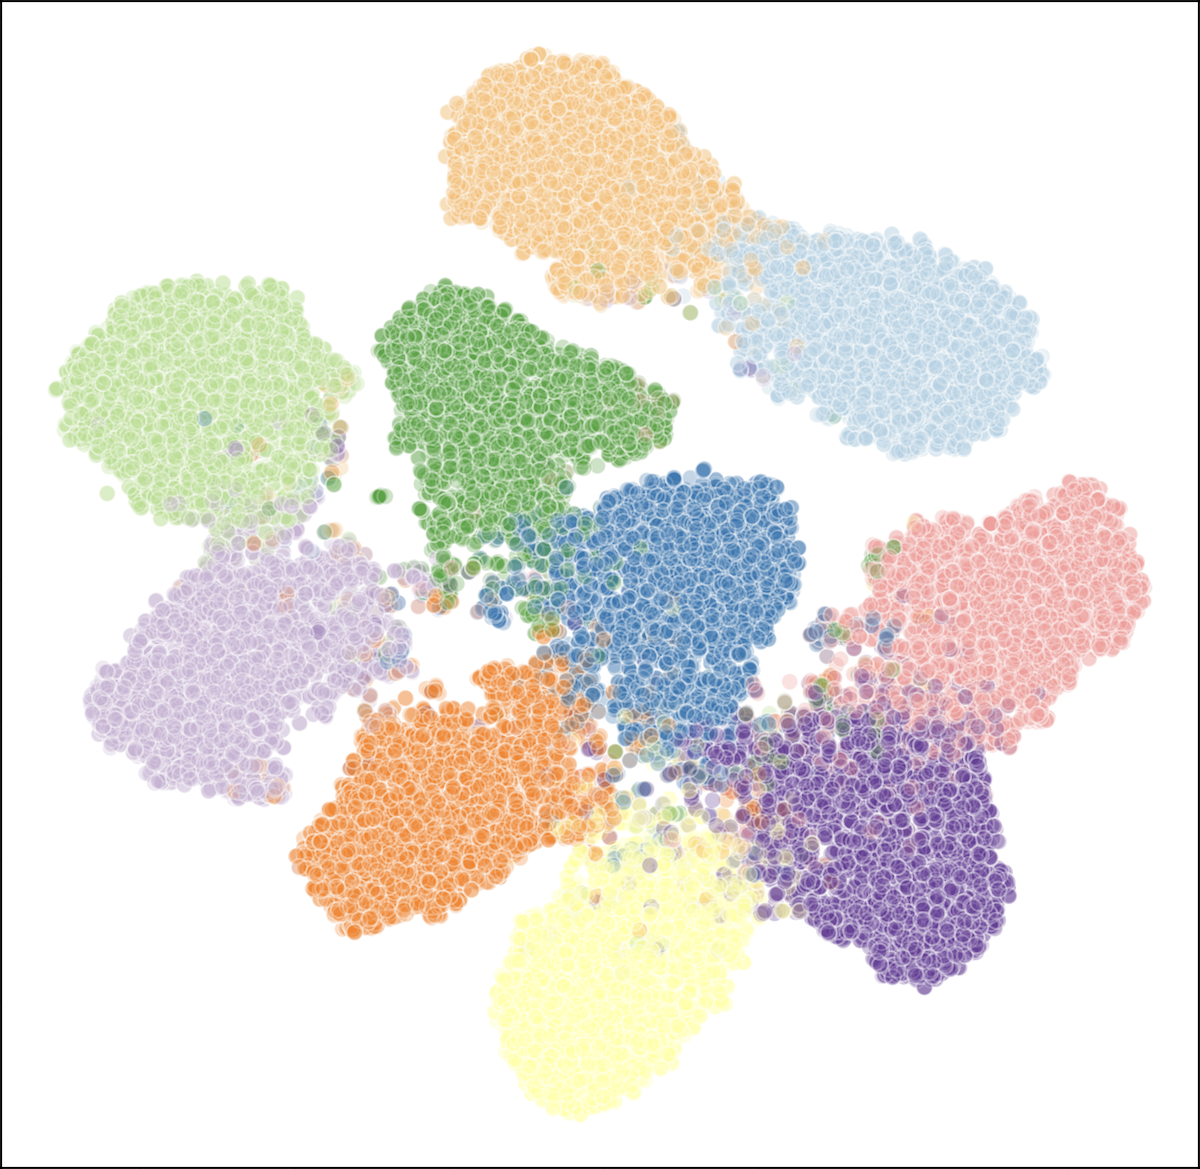
\includegraphics[width=0.45\textwidth]{src/cifar10-tsne.png}}
\subfigure[CIFAR100]{
\label{Fig.sub.a2}
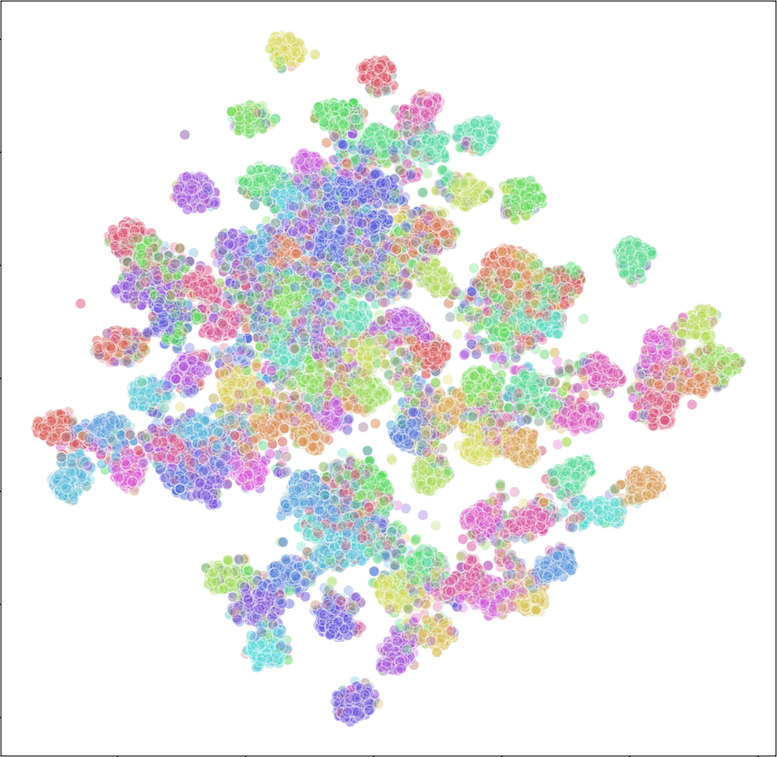
\includegraphics[width=0.45\textwidth]{src/cifar100-tsne.png}}
\caption{Visualisation of extracted features with the t-SNE algorithm.}
\label{Fig.tsne}
\end{figure}

In addition, we compared the training process of the two datasets in Figure \ref{Fig.extracthis}. Across the two training stages, CIFAR10 converges faster than CIFAR100 but it starts to overfit earlier. The green line indicates that we could reduce the number of epochs in the first training stage by half and leave the mining job at the second  stage. 

Finally, we also visualised the classification distributions in Figure \ref{Fig.clscores}. As observed from the quality of blobs plotted in Figure \ref{Fig.tsne}, CIFAR10 samples tend to achieve higher classification scores around 0.9 while CIFAR100 samples are spread across the range below score 0.9. Samples from CIFAR100 are harder to classify correctly with lower scores. Based on the sample selection procedures described in Chapter \ref{bg}, we may need more samples for CIFAR100 to achieve a similar relative accuracy compared with CIFAR10. This suggests that data reduction algorithms may be less efficient for datasets with more classes and lower classification accuracy. We will discuss the algorithm performance further in Section \ref{lr} and \ref{CNN}. 

\begin{figure}[H]
\centering  
\subfigure[CIFAR10]{
\label{Fig.extracthis.a1}
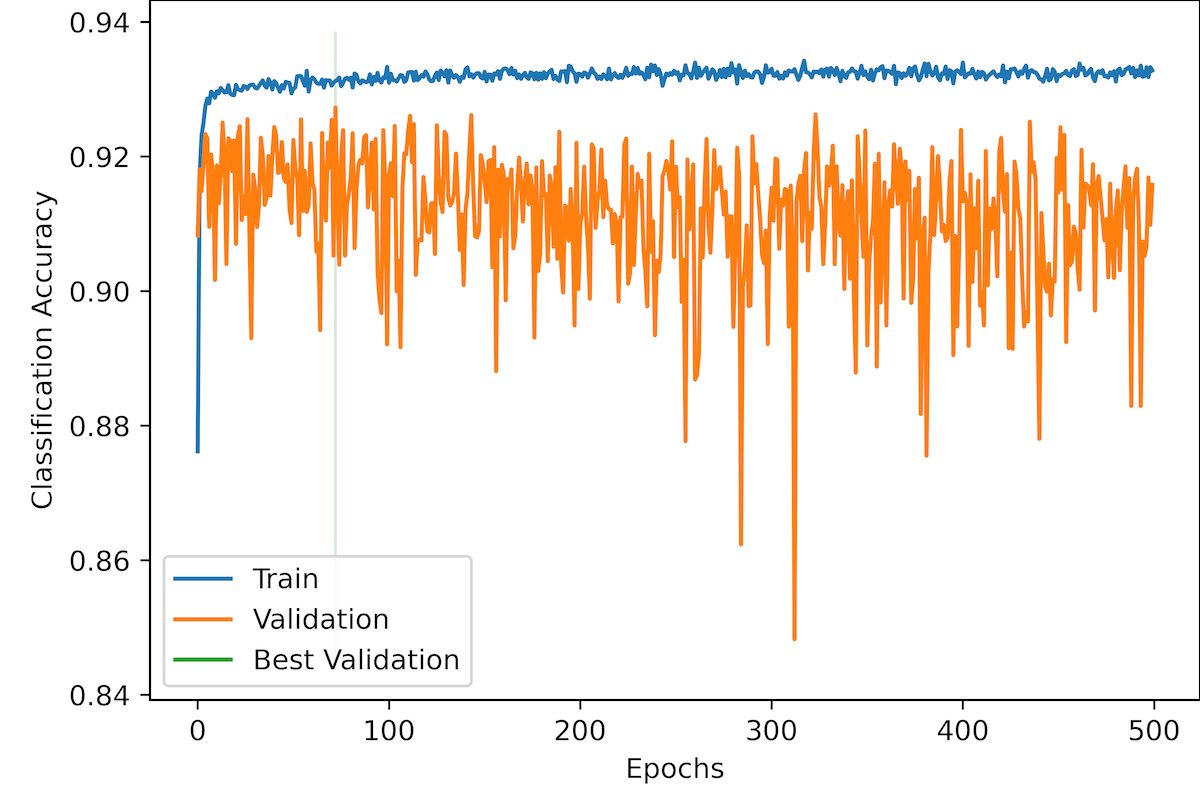
\includegraphics[width=0.45\textwidth]{src/cifar10_exp1_train.png}}
\subfigure[CIFAR10]{
\label{Fig.sub.a2}
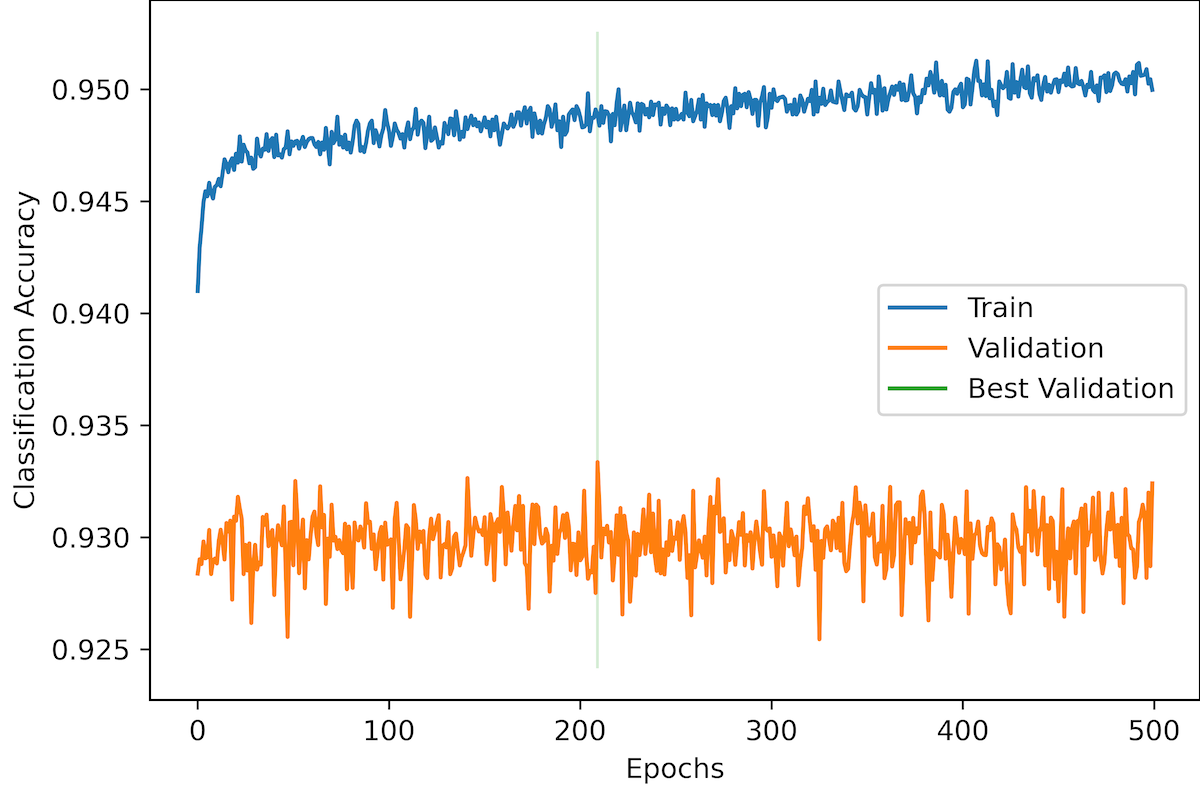
\includegraphics[width=0.45\textwidth]{src/cifar10_exp1_train1.png}}

\subfigure[CIFAR100]{
\label{Fig.sub.a1}
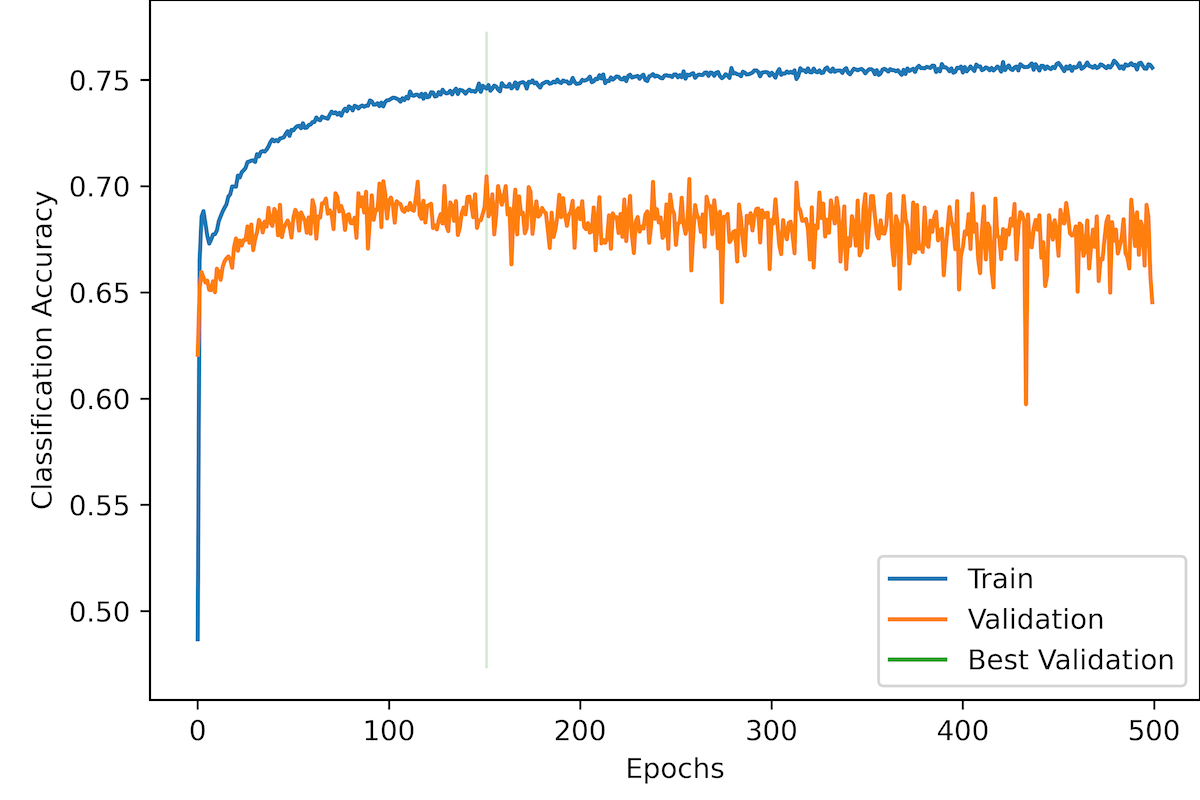
\includegraphics[width=0.45\textwidth]{src/cifar100_exp1_train.png}}
\subfigure[CIFAR100]{
\label{Fig.sub.a2}
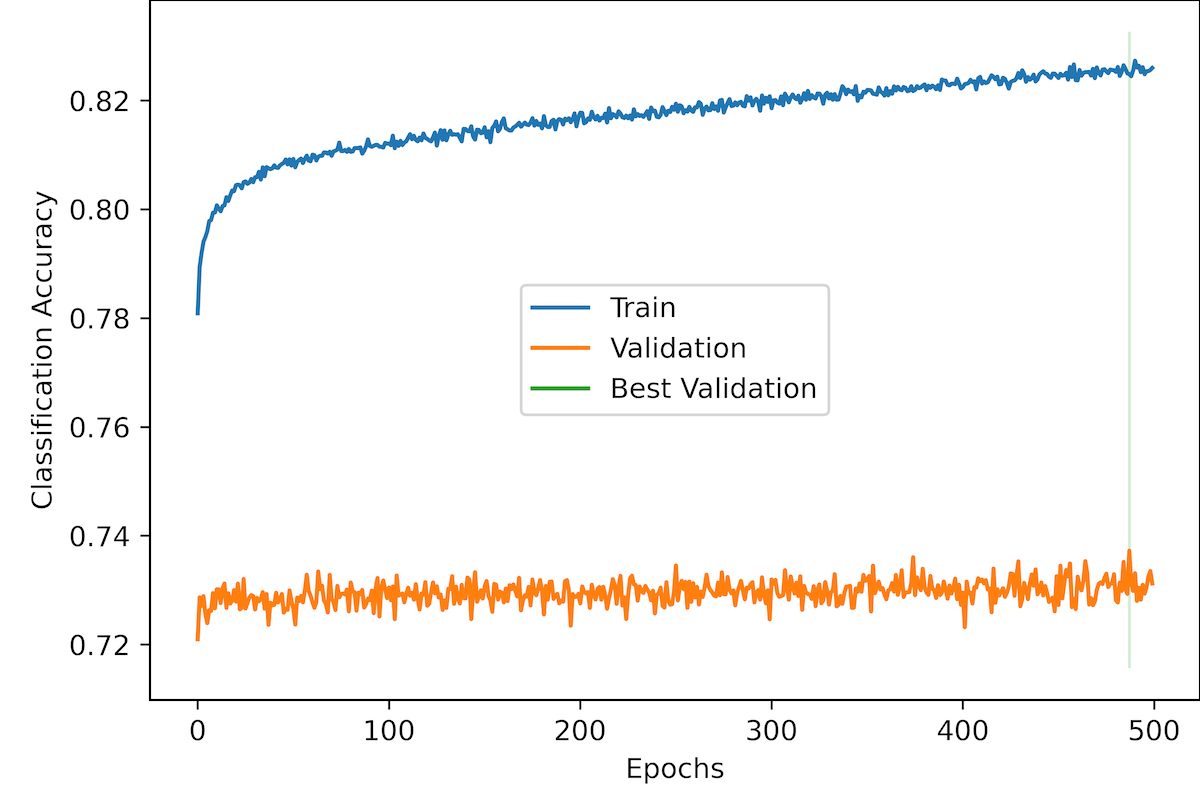
\includegraphics[width=0.45\textwidth]{src/cifar100_exp1_train1.png}}

\caption{The training history of CIFAR10 and CIFAR100. The left column is the first 500 epochs and the right column is the second 500 columns. The green line represents the best validation epoch.}
\label{Fig.extracthis}
\end{figure}

\begin{figure}[H]
\centering  
\subfigure[CIFAR10]{
\label{Fig.sub.a1}
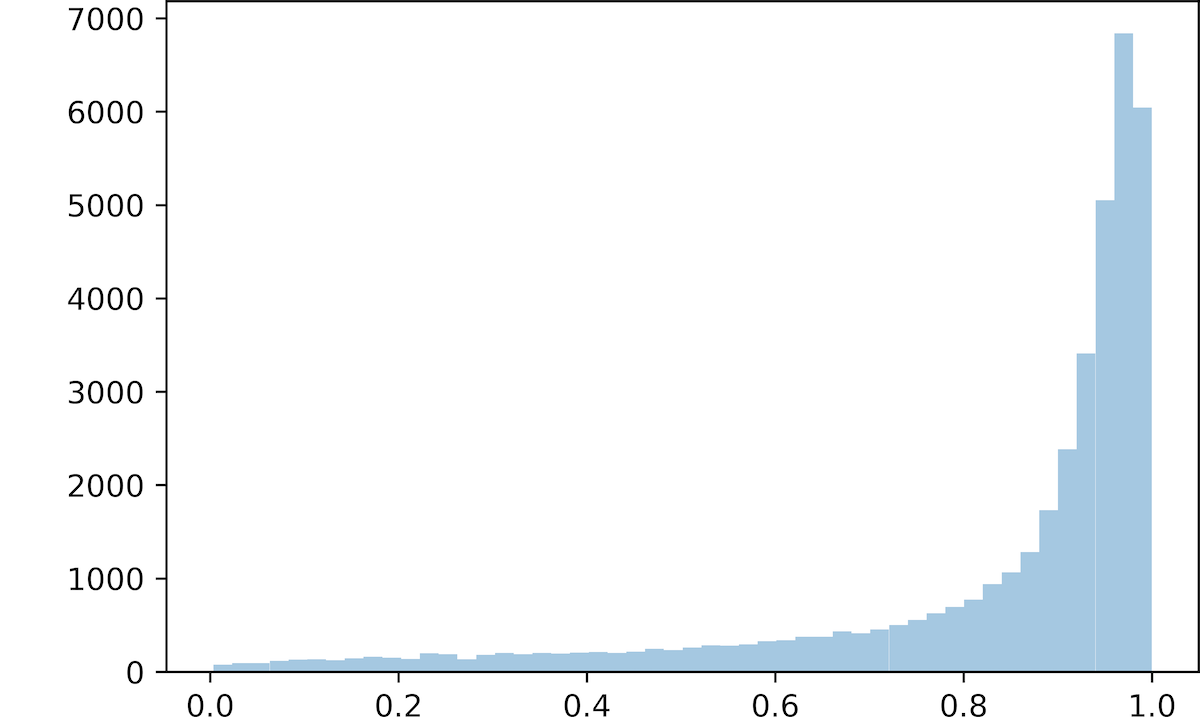
\includegraphics[width=0.45\textwidth]{src/cl_score_cifar10.png}}
\subfigure[CIFAR100]{
\label{Fig.sub.a2}
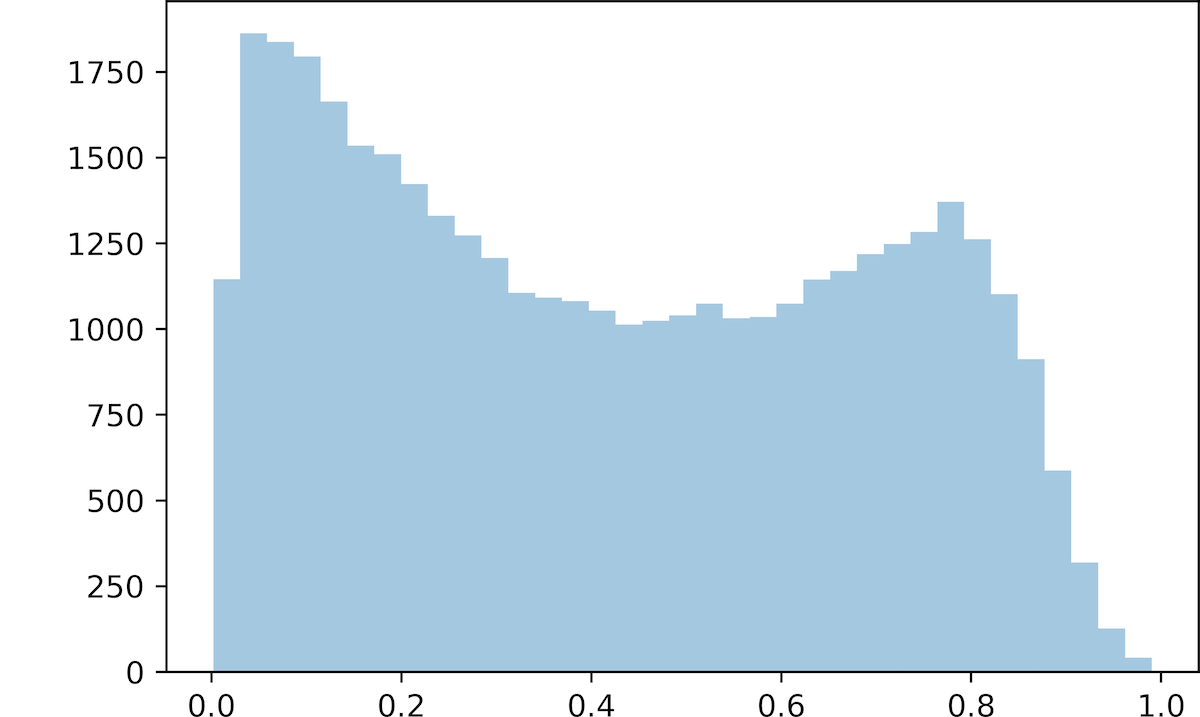
\includegraphics[width=0.45\textwidth]{src/cl_score_cifar100.png}}
\caption{Classification score distributions}
\label{Fig.clscores}
\end{figure}





\section{Experiment 2: Intrinsic Behaviour}
Obtaining the  with  In this section, we use CIFAR10 to show the intrinsic behaviour of each data reduction algorithm for the reason that the quality of t-SNE projected blobs are better than CIFAR100 thus we can visualise the selection preference easily. 

For POP, we can tune the difference tolerance.   
\begin{figure}[H]
\centering  
\subfigure[T=1, 8701 samples]{
\label{Fig.sub.a1}
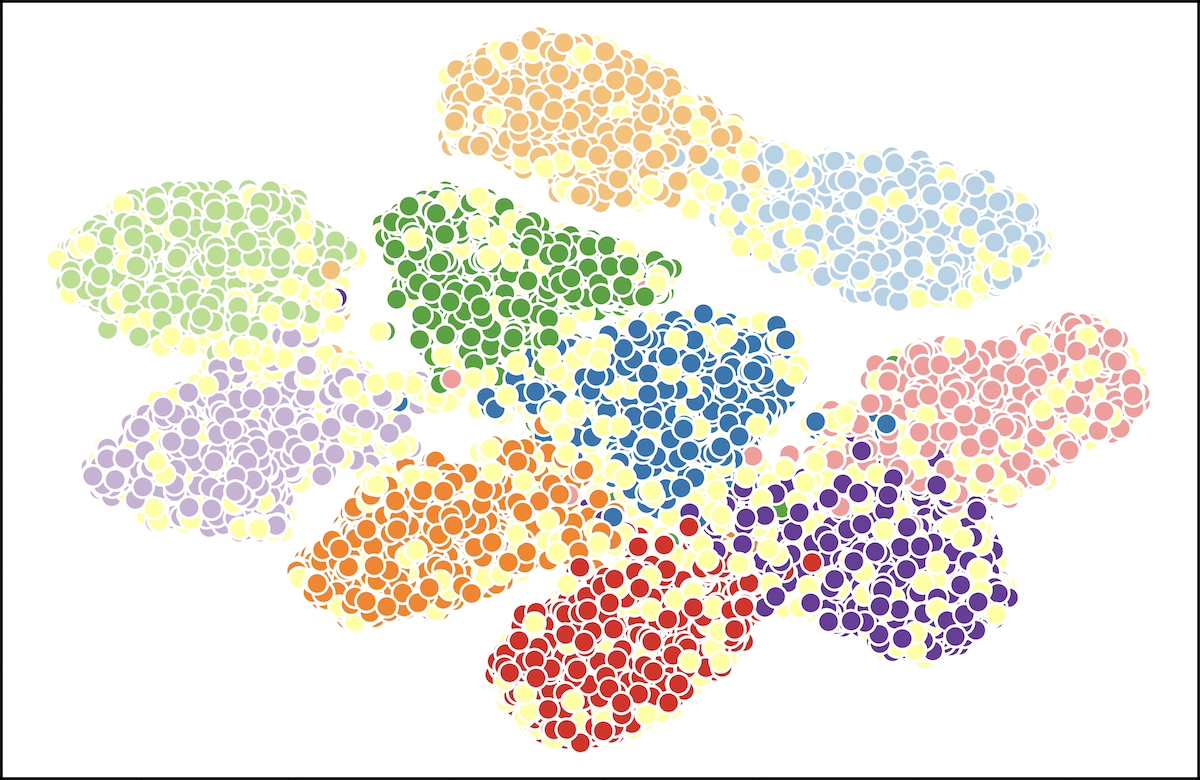
\includegraphics[width=0.32\textwidth]{src/pop-cifar10-1.png}}
\subfigure[T=0.5, 14111 samples]{
\label{Fig.sub.a2}
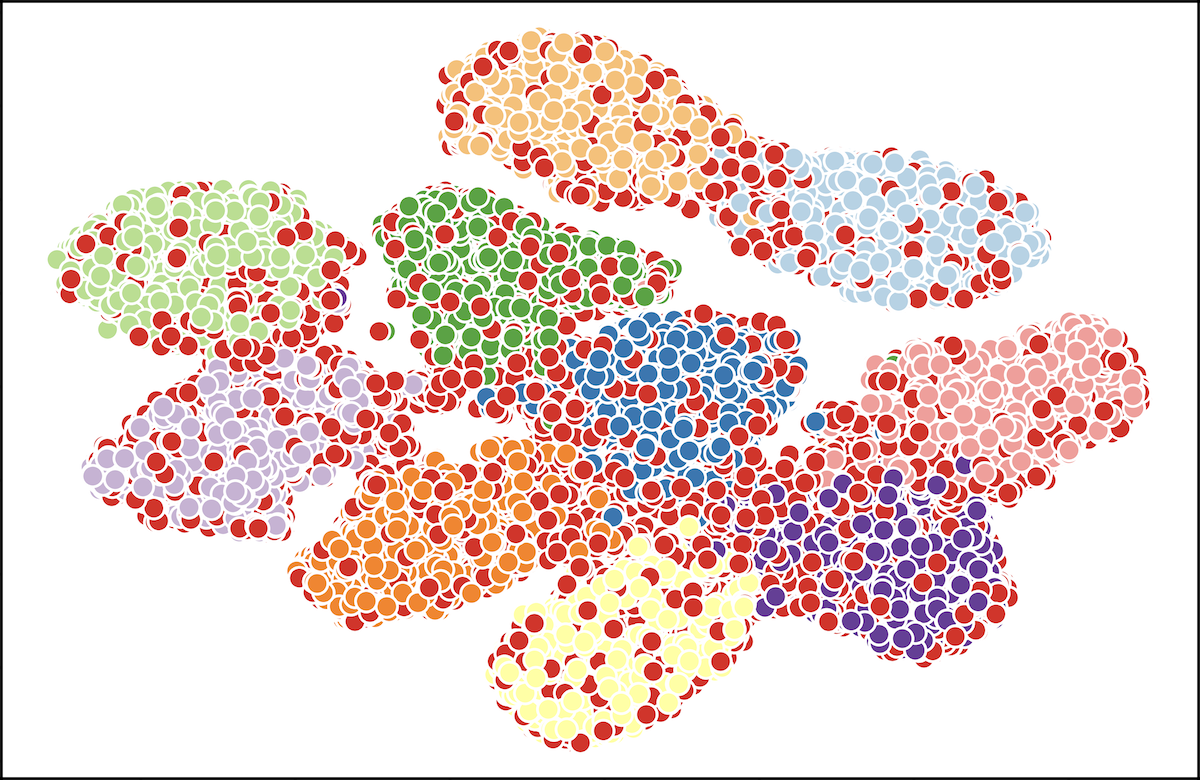
\includegraphics[width=0.32\textwidth]{src/pop-cifar10-5.png}}
\subfigure[T=0.1, 31966 samples]{
\label{Fig.sub.a1}
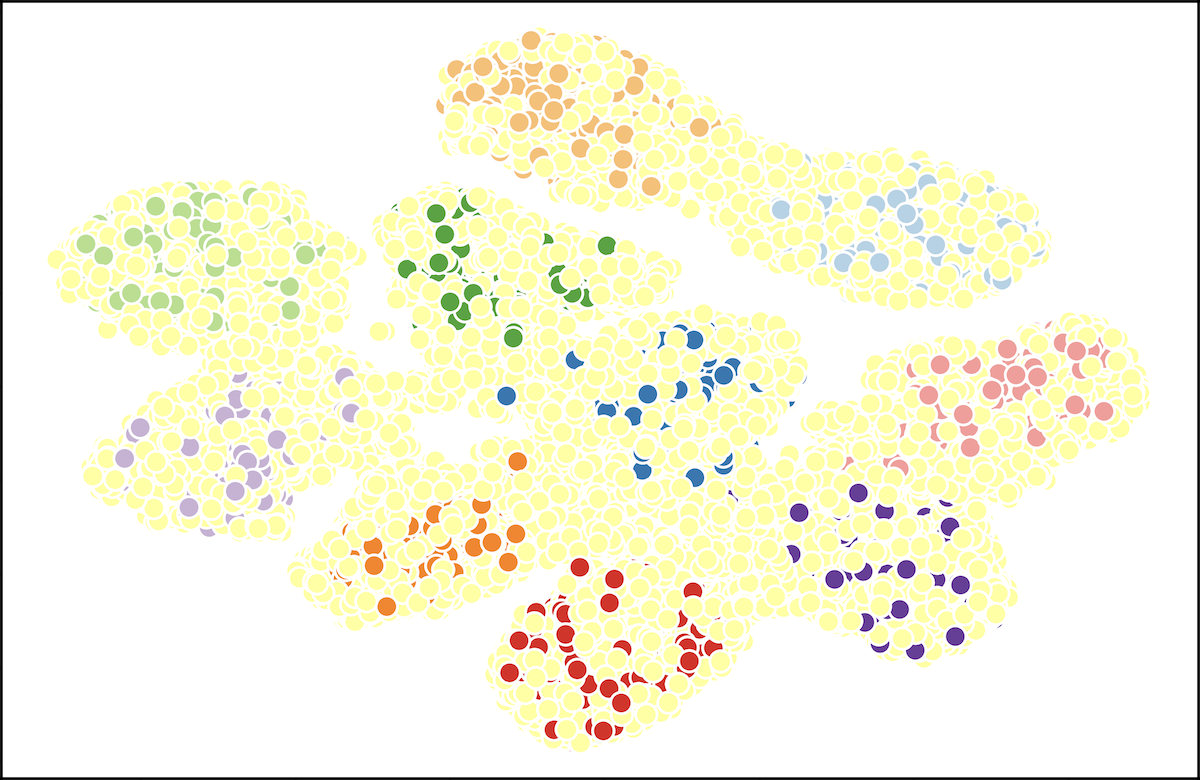
\includegraphics[width=0.32\textwidth]{src/pop-cifar10-01.png}}
\caption{POP tune threshold}
\label{Fig.popcifar10}
\end{figure}

For EGDIS, we can tune the k of the k-NN classifier.
\begin{figure}[H]
\centering  
\subfigure[k=7, 2799 samples]{
\label{Fig.sub.a1}
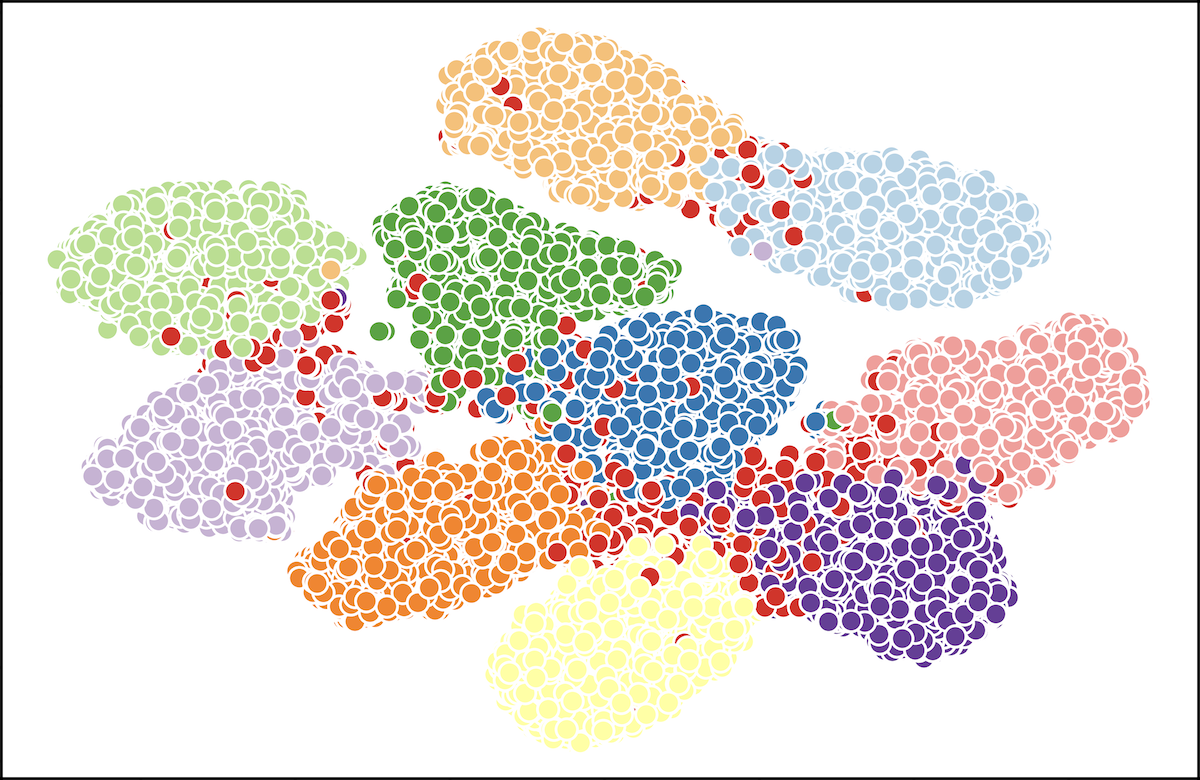
\includegraphics[width=0.32\textwidth]{src/egdis-cifar10-8.png}}
\subfigure[k=5, 3483 samples]{
\label{Fig.sub.a2}
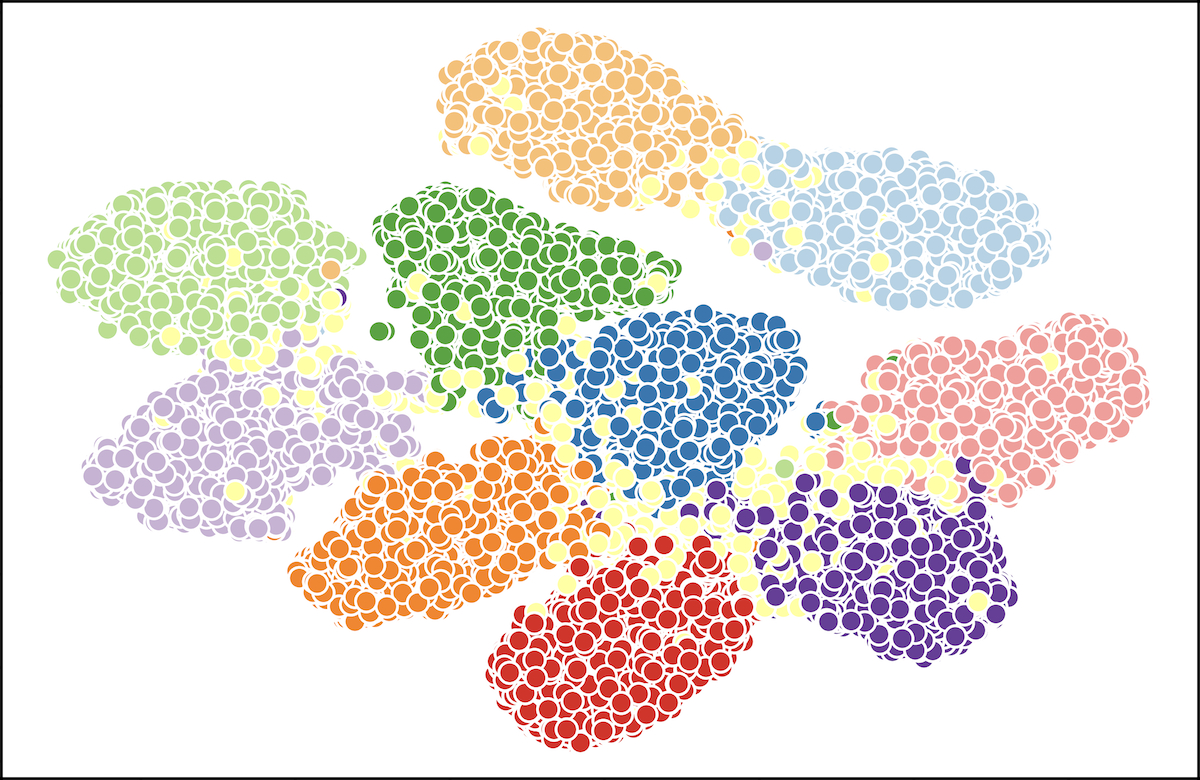
\includegraphics[width=0.32\textwidth]{src/egdis-cifar10-6.png}}
\subfigure[k=3, 5966 samples]{
\label{Fig.sub.a1}
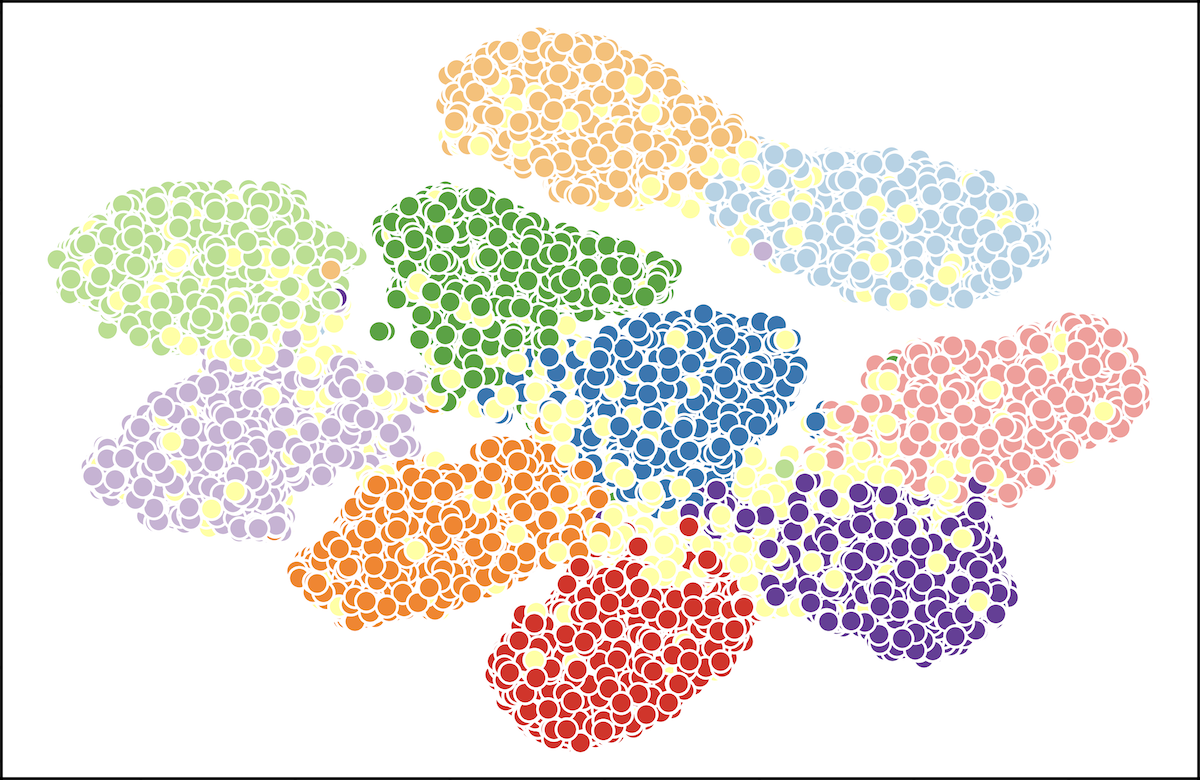
\includegraphics[width=0.32\textwidth]{src/egdis-cifar10-4.png}}
\caption{EGDIS tune kNN}
\label{Fig.egdiscifar10}
\end{figure}


For CL, we can tune the number of samples selected.

\begin{figure}[H]
\centering  
\subfigure[P=10\%, 4000 samples]{
\label{Fig.sub.a1}
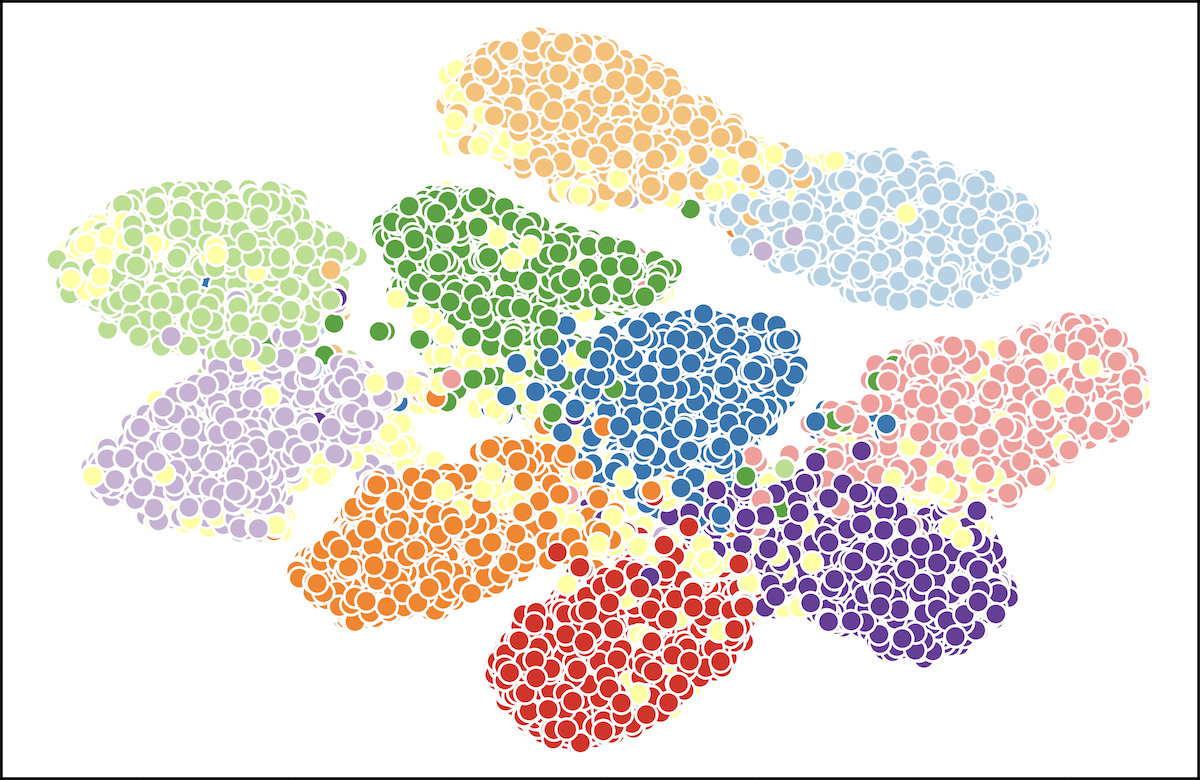
\includegraphics[width=0.32\textwidth]{src/cl-cifar10-1.png}}
\subfigure[P=30\%, 12000 samples]{
\label{Fig.sub.a2}
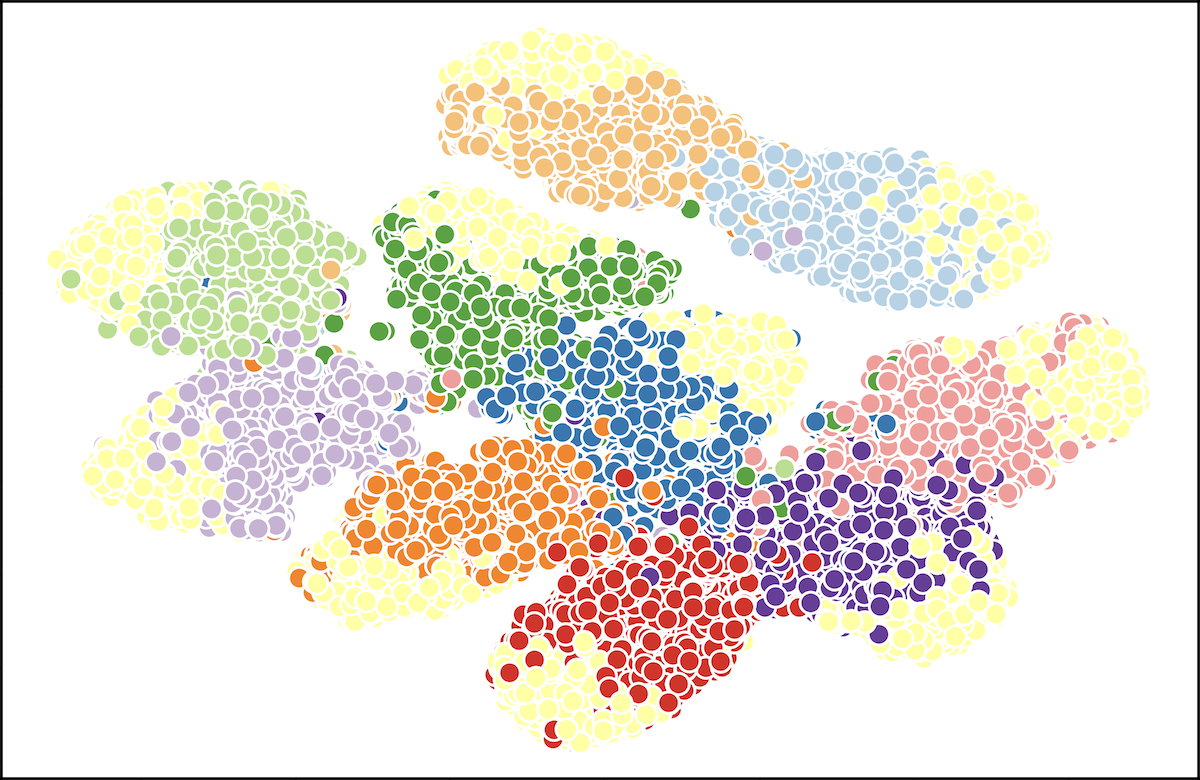
\includegraphics[width=0.32\textwidth]{src/cl-cifar10-3.png}}
\subfigure[P=50\%, 20000 samples]{
\label{Fig.sub.a1}
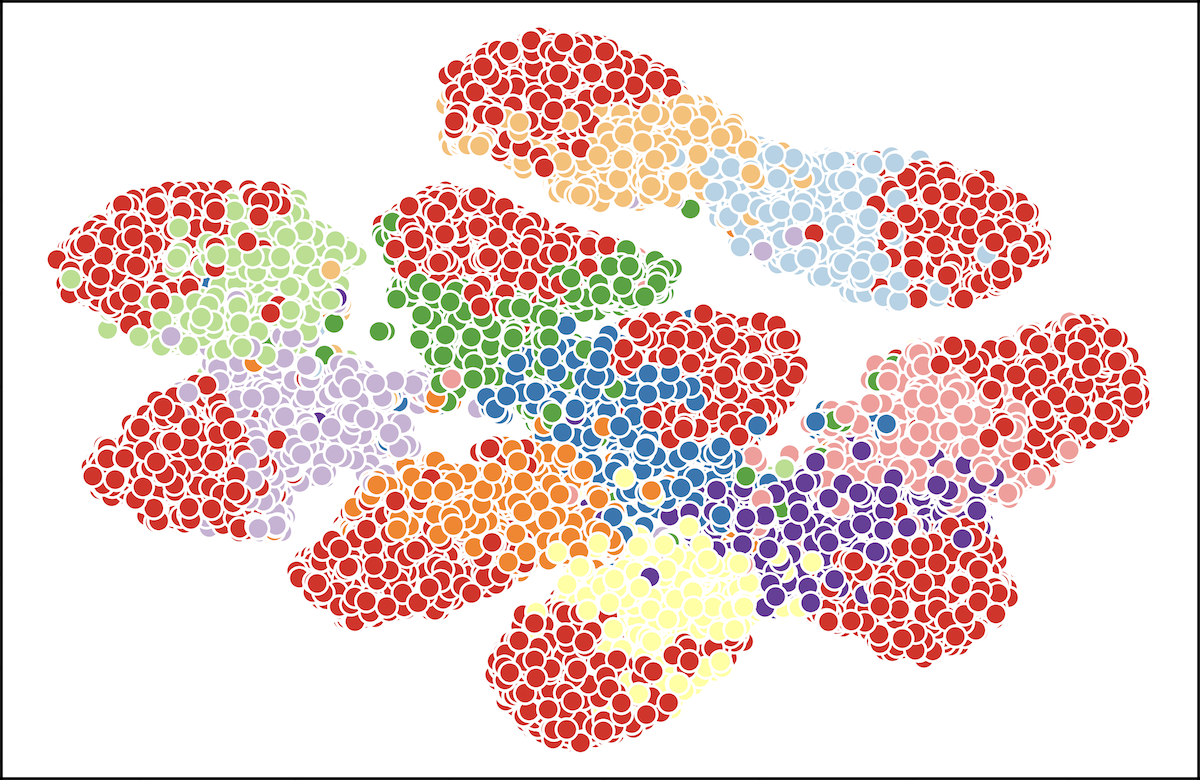
\includegraphics[width=0.32\textwidth]{src/cl-cifar10-5.png}}
\caption{CL tune selection percentage}
\label{Fig.clcifar10}
\end{figure}
For WCL, we can tune the difficulty sample portion.

WCL which takes the sample within each class based on the sample score. Although most samples are selected from the high score region, there are some sample selected from the low score region. The problem is that for relatively easy dataset like CIFAR10, the behaviour is close to random selection because most samples have a score higher than 0.8. The score distribution is shown below.

\begin{figure}[H]
\centering  
\subfigure[CIFAR10]{
\label{Fig.sub.a1}
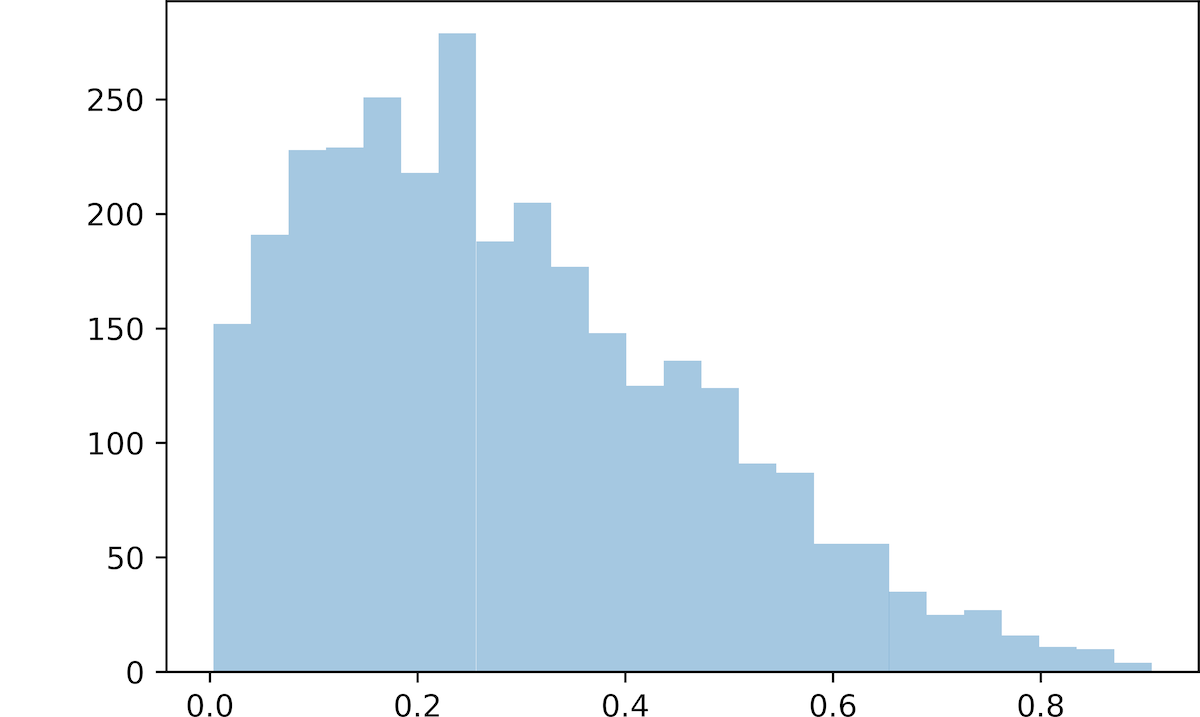
\includegraphics[width=0.45\textwidth]{src/boundarydis-cifar10-dis.png}}
\subfigure[CIFAR100]{
\label{Fig.sub.a2}
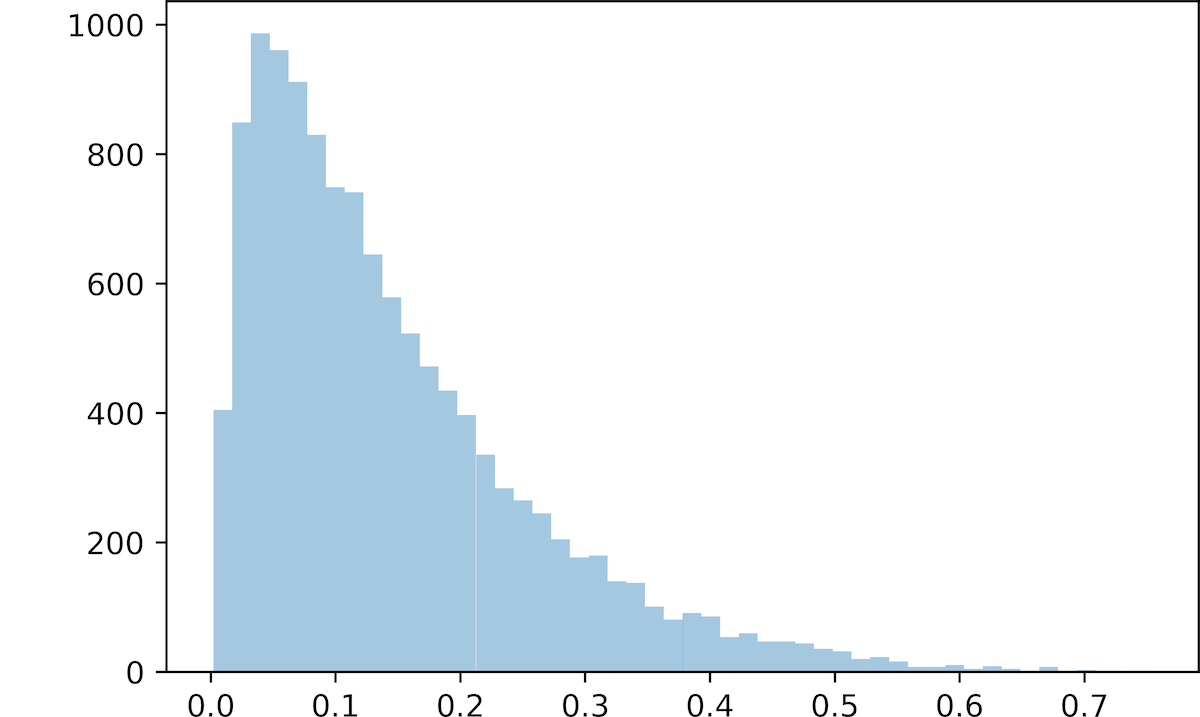
\includegraphics[width=0.45\textwidth]{src/boundarydis-cifar100-dis.png}}
\caption{EGDIS boundary score distribution}
\label{Fig.egdisboscores}
\end{figure}

\begin{figure}[H]
\centering  
\subfigure[P=10\%, 4000 samples]{
\label{Fig.sub.a1}
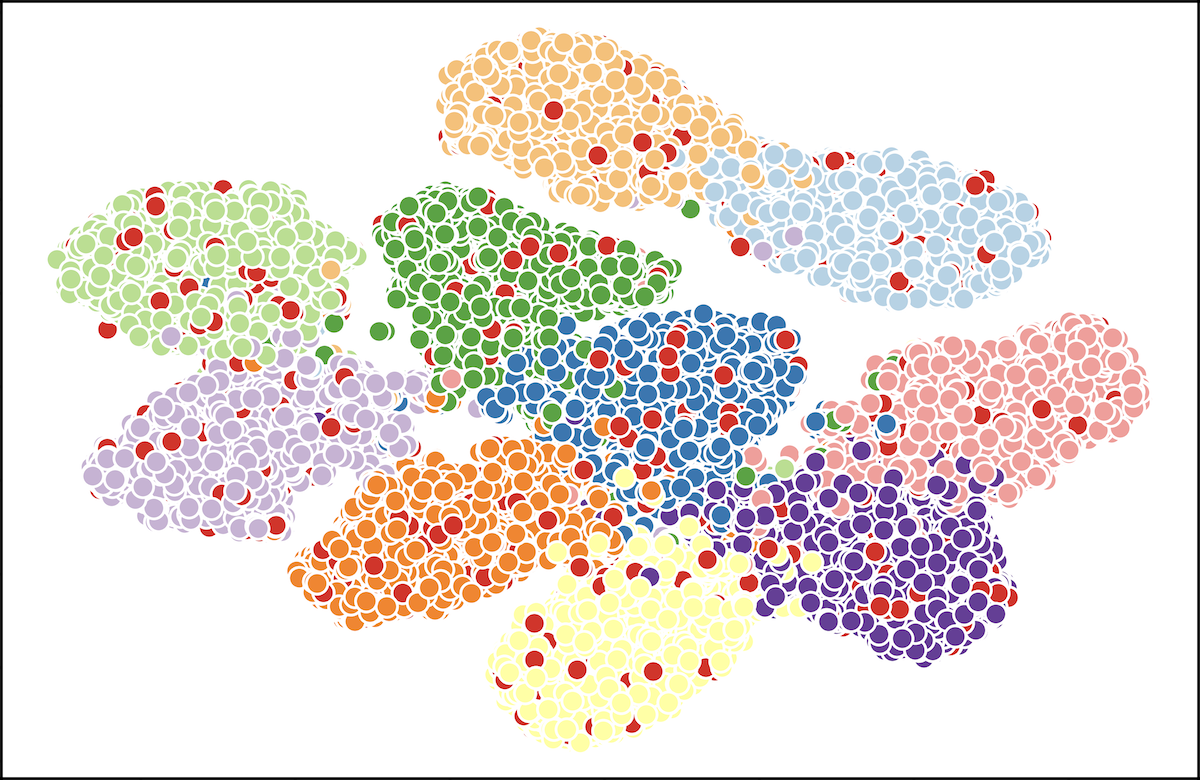
\includegraphics[width=0.32\textwidth]{src/wcl-cifar10-1.png}}
\subfigure[P=30\%, 12000 samples]{
\label{Fig.sub.a2}
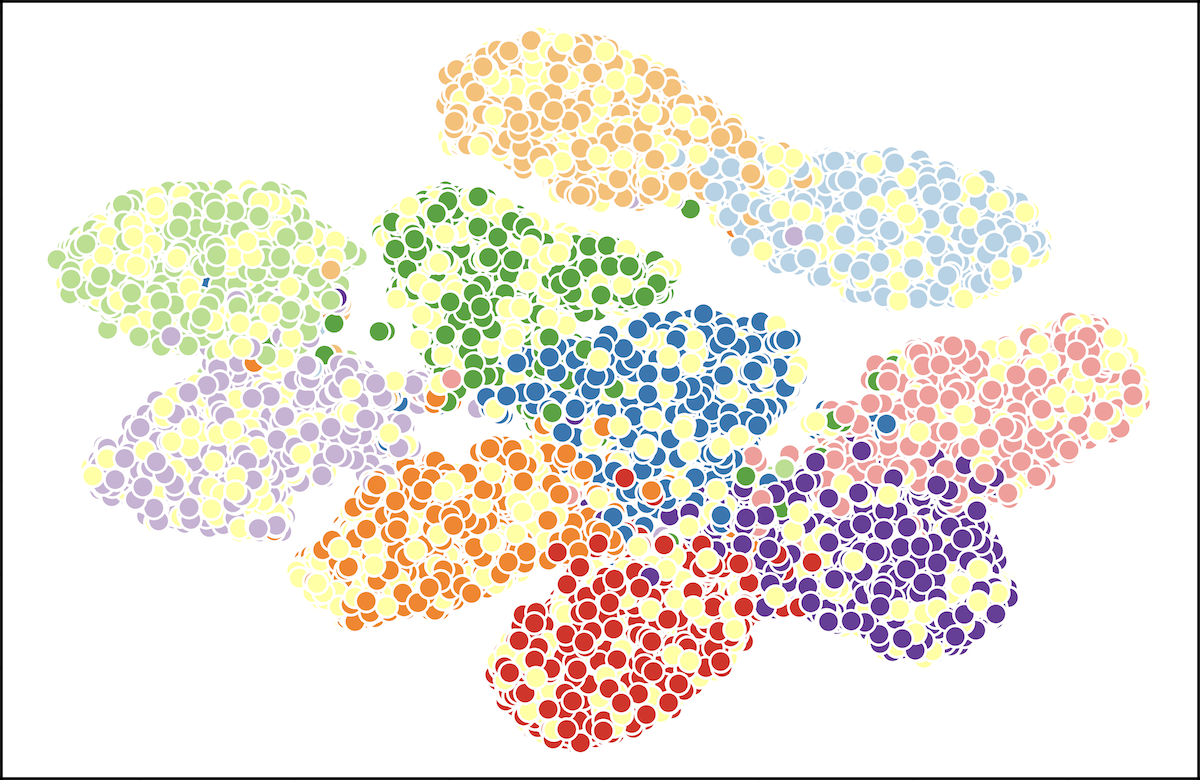
\includegraphics[width=0.32\textwidth]{src/wcl-cifar10-3.png}}
\subfigure[P=50\%, 20000 samples]{
\label{Fig.sub.a1}
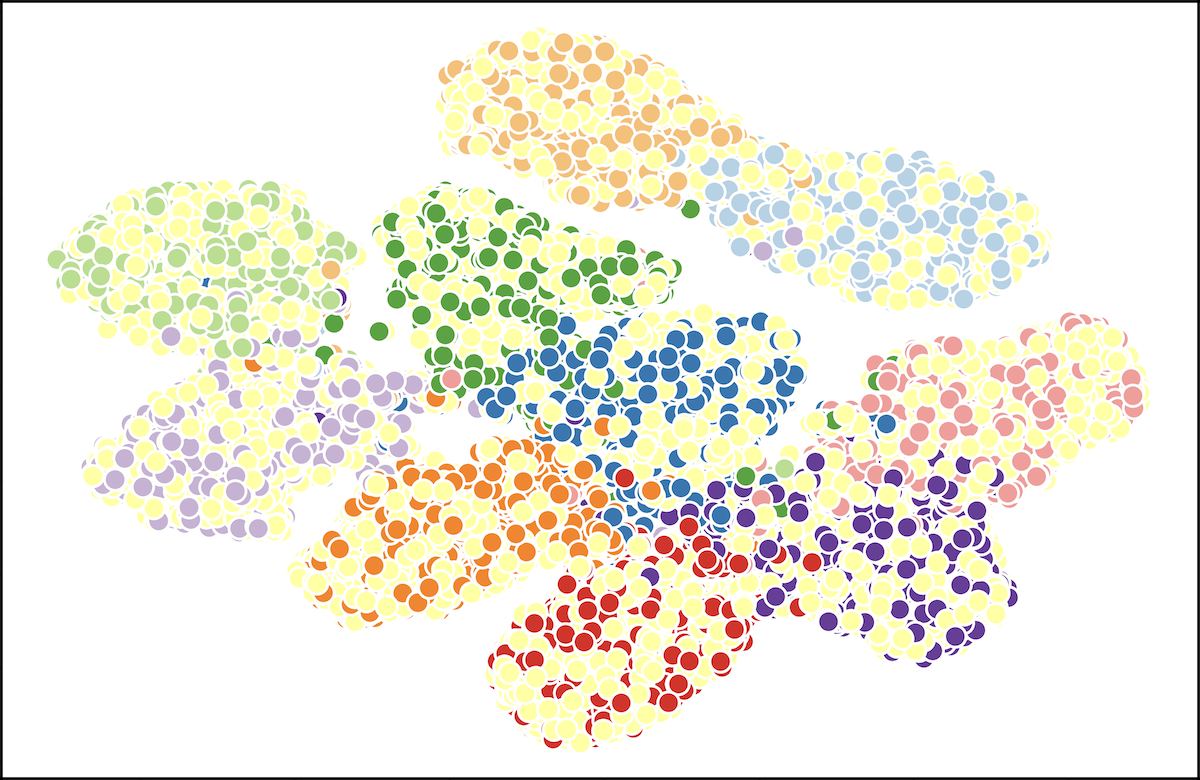
\includegraphics[width=0.32\textwidth]{src/wcl-cifar10-5.png}}

\subfigure[P=10\%, 4000 samples]{
\label{Fig.sub.a1}
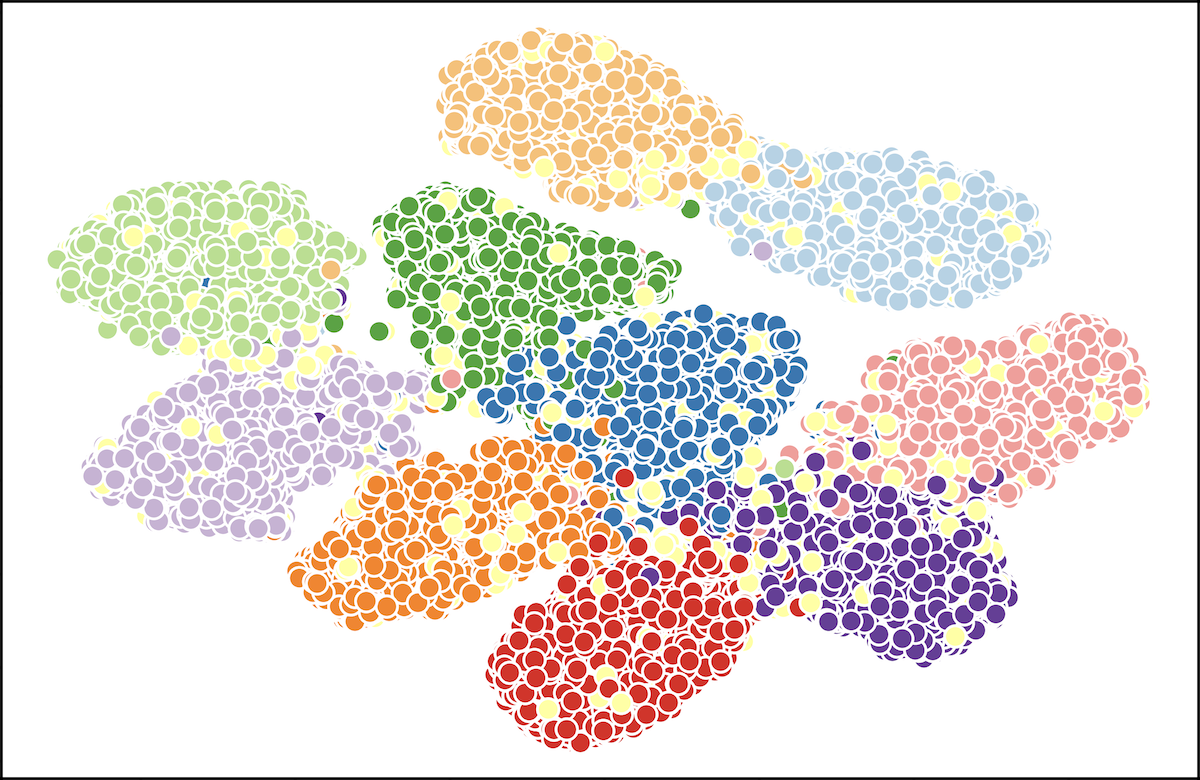
\includegraphics[width=0.32\textwidth]{src/wcl2-cifar10-1.png}}
\subfigure[P=30\%, 12000 samples]{
\label{Fig.sub.a2}
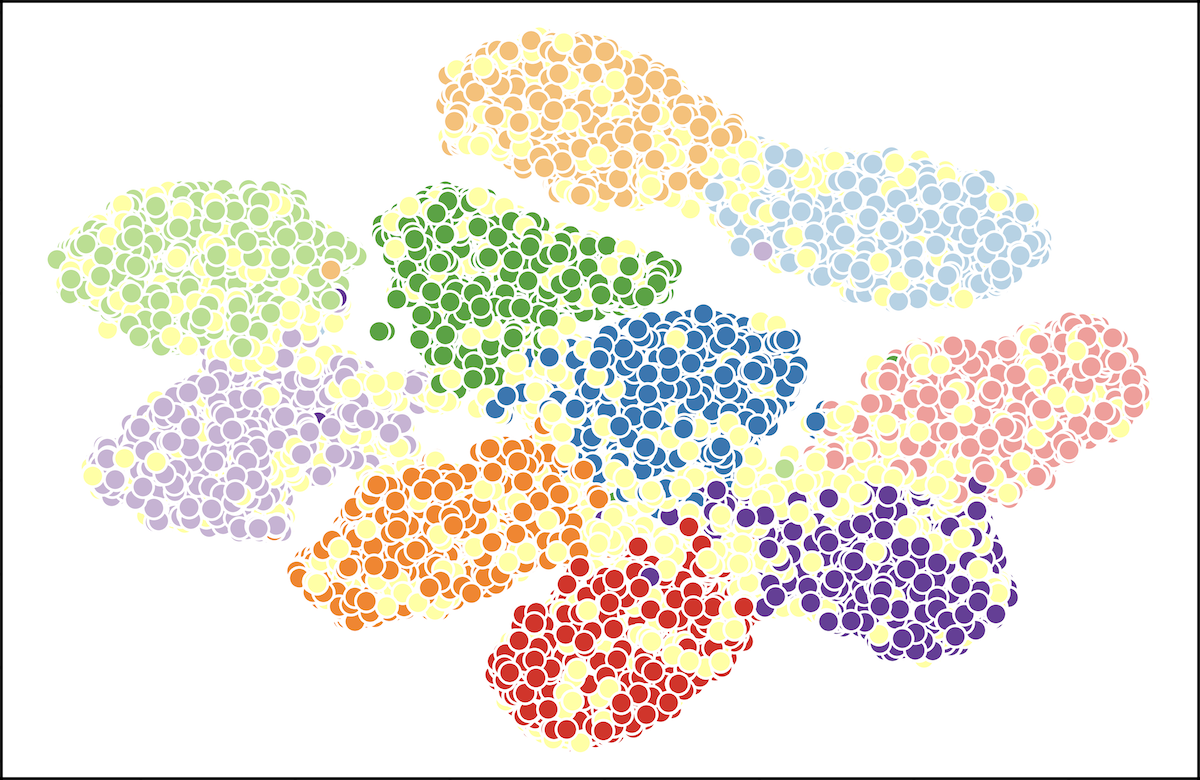
\includegraphics[width=0.32\textwidth]{src/wcl2-cifar10-3.png}}
\subfigure[P=50\%, 20000 samples]{
\label{Fig.sub.a1}
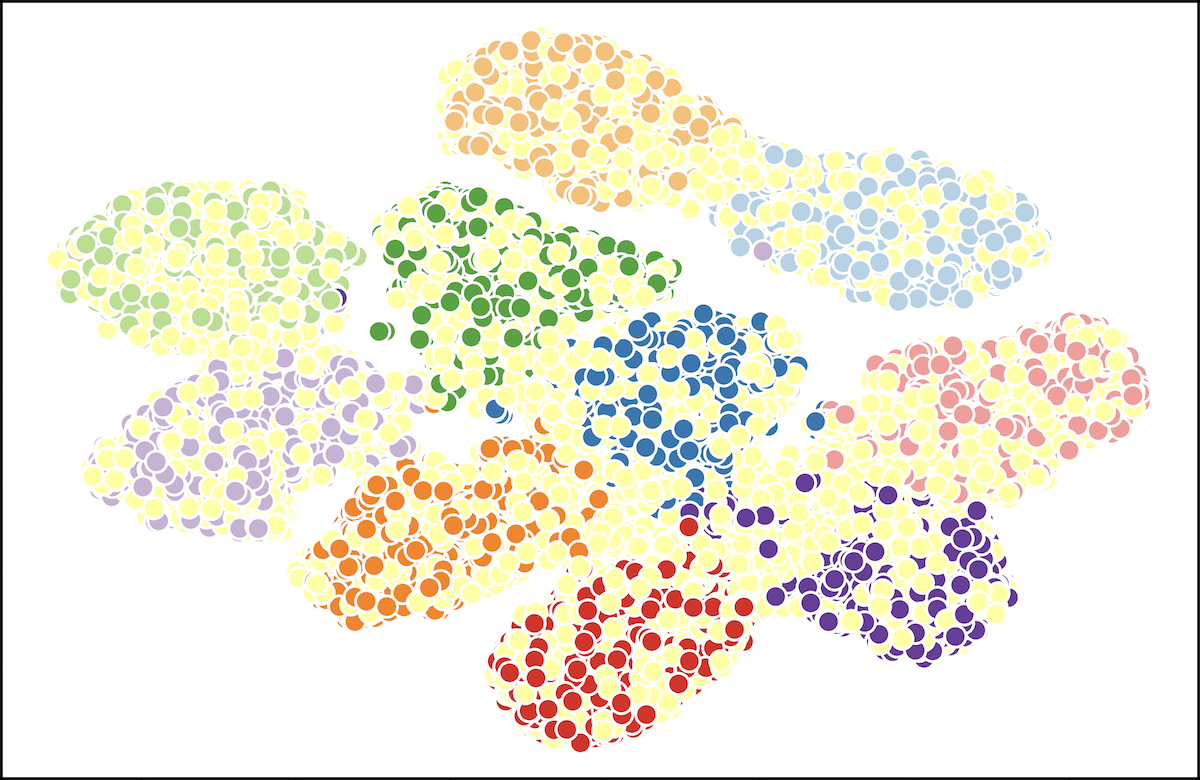
\includegraphics[width=0.32\textwidth]{src/wcl2-cifar10-5.png}}
\caption{WCL tune selection percentage. The first row we use weighted sampling method, the second row we use EGDIS based method.}
\label{Fig.clcifar10}
\end{figure}

In theory, POP tends to select pure boundary samples. EGDIS tends to select samples near two closing clusters and the samples from densest area, which could be anywhere actually. For CL, it tends to select samples far from the boundary, i.e the inner samples. WCL, would choose sample from both the closer cluster boundaries as well as the inner samples. The drawback of CL is that when all the samples are simple enough, with score larger than 0.9, they would tend to act like random selection.



\section{Experiment 3: Logistic Regression}
\label{lr}
We choose 40 and 20 as the number of our extra synthesised datasets, with LR accuracy: 0.78925, 0.853. By fine-tuning the selected subsets, the test accuracy is: 0.8065, 0.8745.

 \begin{figure}[H]
 \centering
 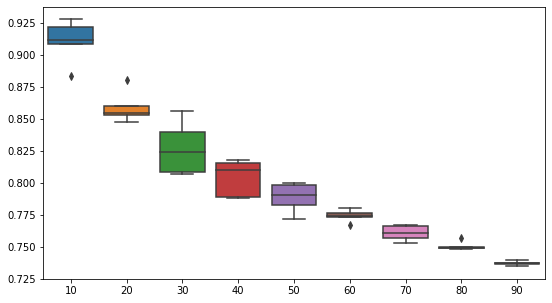
\includegraphics[width=0.8\textwidth]{src/subsets.png}
 \caption{The test set accuracies of CIFAR100 subsets. Horizontal axis is the number of classes selected. Vertical axis is the accuracy score. For each selection, we randomly choose the classes for five times and report the accuracy with logistic regression model.}
 \label{Fig.logistic_subsets}
 \end{figure}
 
 \begin{figure}[H]
\centering  
\subfigure[CIFAR10, 40000 samples]{
\label{Fig.sub.a1}
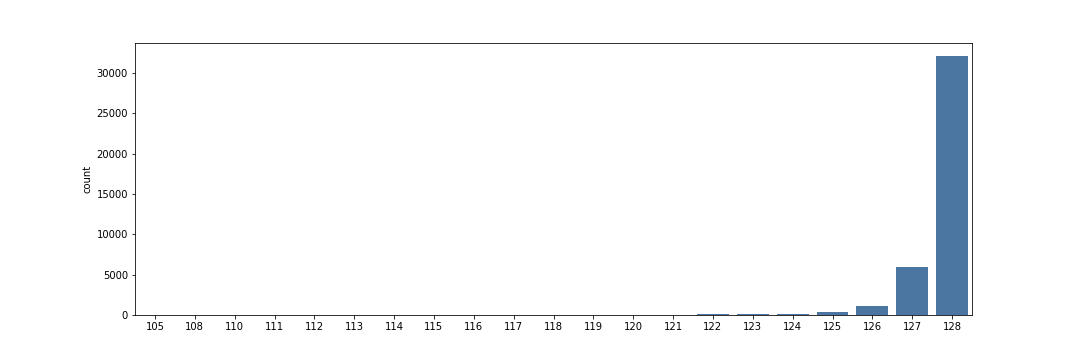
\includegraphics[width=1\textwidth]{src/pop-cifar10-count.png}}
\subfigure[CIFAR20, 8028 samples]{
\label{Fig.sub.a2}
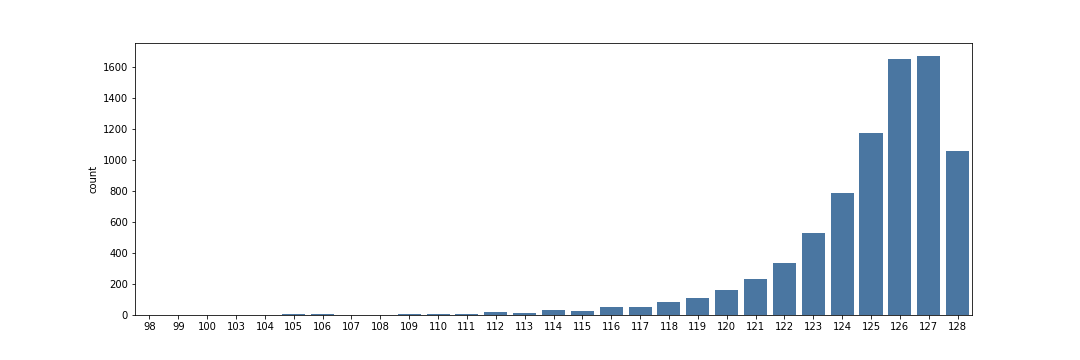
\includegraphics[width=1\textwidth]{src/pop-cifar20-count.png}}
\subfigure[CIFAR40, 16042 samples]{
\label{Fig.sub.a1}
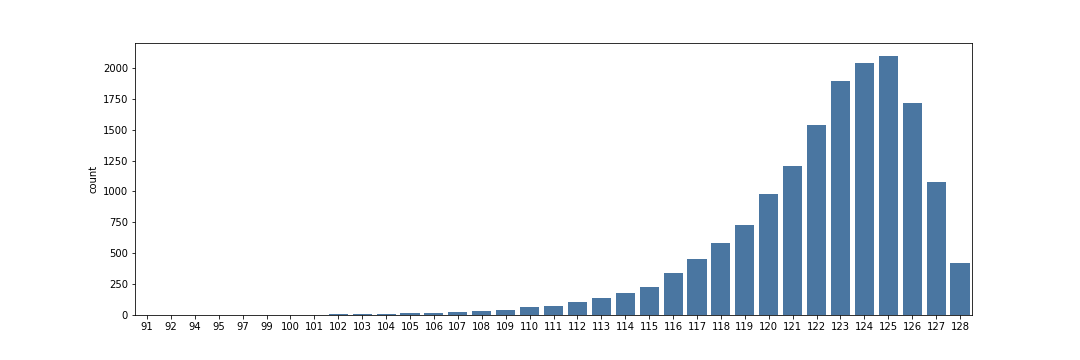
\includegraphics[width=1\textwidth]{src/pop-cifar40-count.png}}
\subfigure[CIFAR100, 40000 samples]{
\label{Fig.sub.a1}
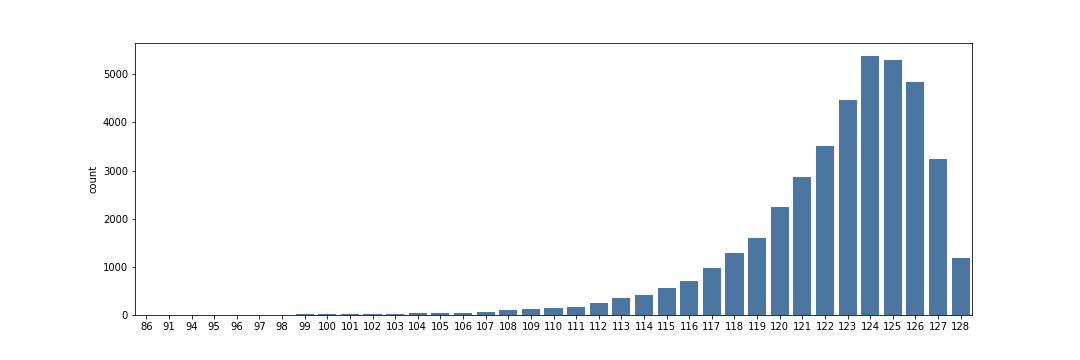
\includegraphics[width=1\textwidth]{src/pop-cifar100-count.png}}
\caption{POP with 4 datasets.}
\label{Fig.clcifar10}
\end{figure}

Even for POP with threshold 1, the number of pure inner is still low. Therefore, it is not good to choose samples with weakness < 128. We fix the number and choose CIFAR samples. From our experiment, we found that the relative accuracy acquired from EGDIS is good enough. Therefore, we make POP to select the same amount of samples as EGDIS, by ranking POP samples based on weakness, to compare their performance.
 
 
\begin{table}
    \centering
    \begin{tabular}{|l|l|l|l|l|l|l|}
    \hline
        Datasets & Retention Rate  & POP & EGDIS & CL & WCL & BWCL \\ \hline
        CIFAR10 & 14.915\% & 100.00\% & \textbf{100.04}\% & 99.74\% & 99.96\% & 99.91\% \\ \hline
        CIFAR20 & 16.67\% & \textbf{99.94}\% & 99.01\% & 99.57\% & 99.31\% & 99.43\% \\ \hline
        CIFAR40 & 21.09\% & \textbf{99.64}\% & 98.92\% & 99.09\% & 99.46\% & 99.63\% \\ \hline
        CIFAR100 & 31.48\% & 99.38\% & 97.78\% & 98.78\% & 99.46\% & \textbf{99.49}\% \\ \hline
    \end{tabular}
    \caption{Logistic Regression test set relative accuracy by averaging 12 runs}
    \label{132e3213}
\end{table}


\begin{figure}[H]
\centering  
\subfigure[Relative Accuracy]{
\label{Fig.sub.a1}
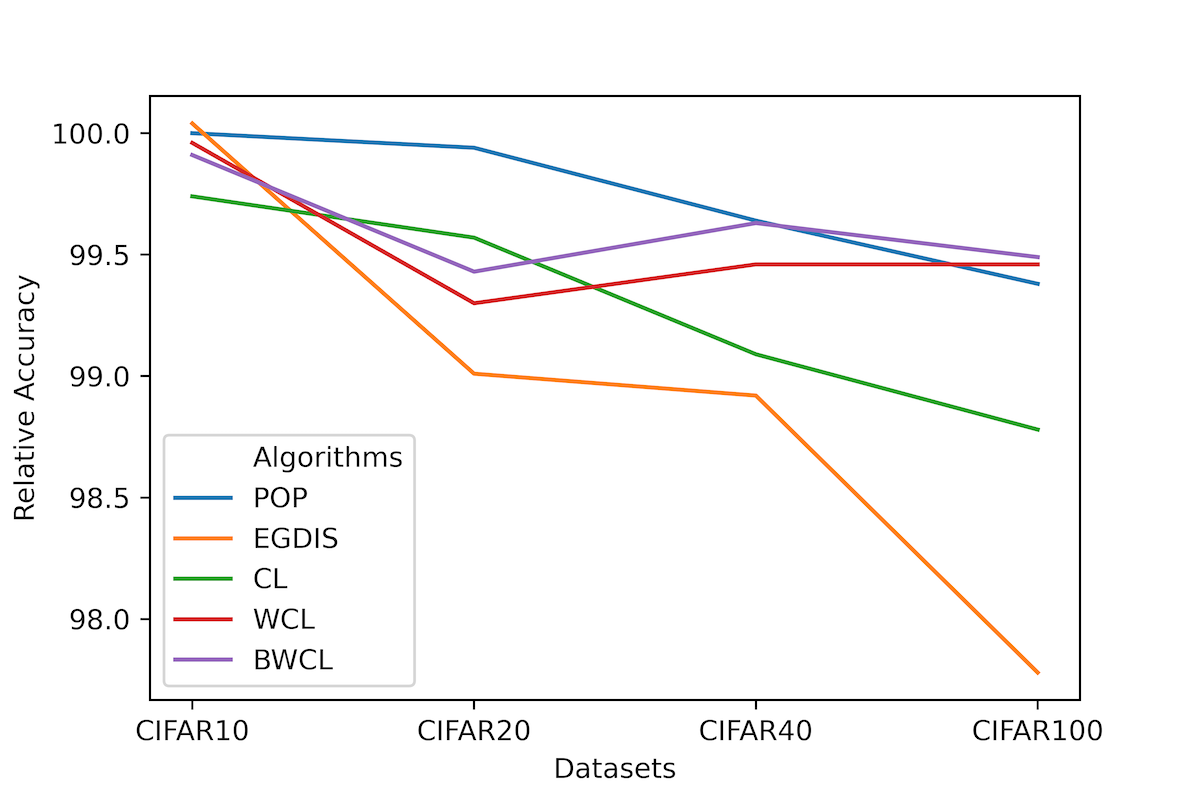
\includegraphics[width=0.45\textwidth]{src/lg_relative.png}}
\subfigure[Relative Accuracy of BWCL by tuning maximum boundary proportion]{
\label{Fig.sub.a2}
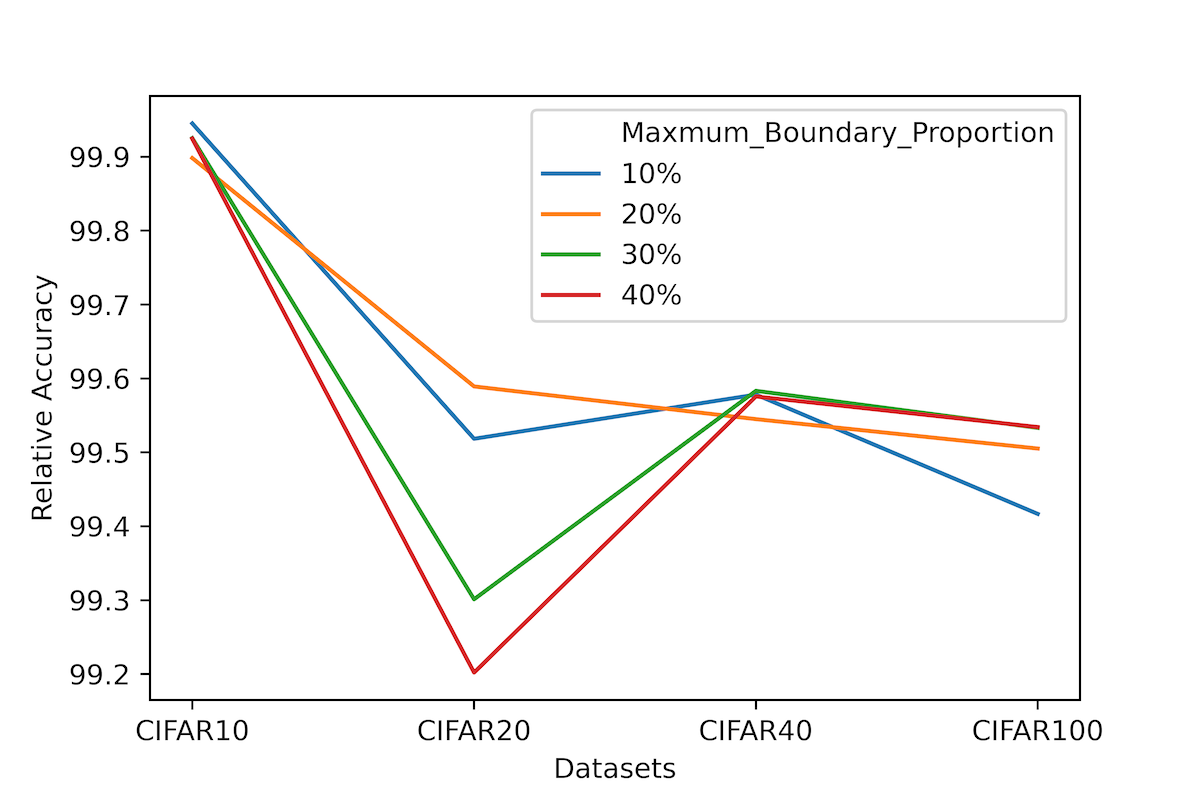
\includegraphics[width=0.45\textwidth]{src/bwcl_relative.png}}
\caption{Relative Accuracy of data reduction algorithms}
\label{Fig.logistic_relativeacc}
\end{figure}

However, this is not a solid conclusion because the quality of the extracted features are so good that the classes are classified easily. We show this effect by varying the proportion of samples selected with BWCL, 0.4.

\begin{figure}[H]
 \centering
 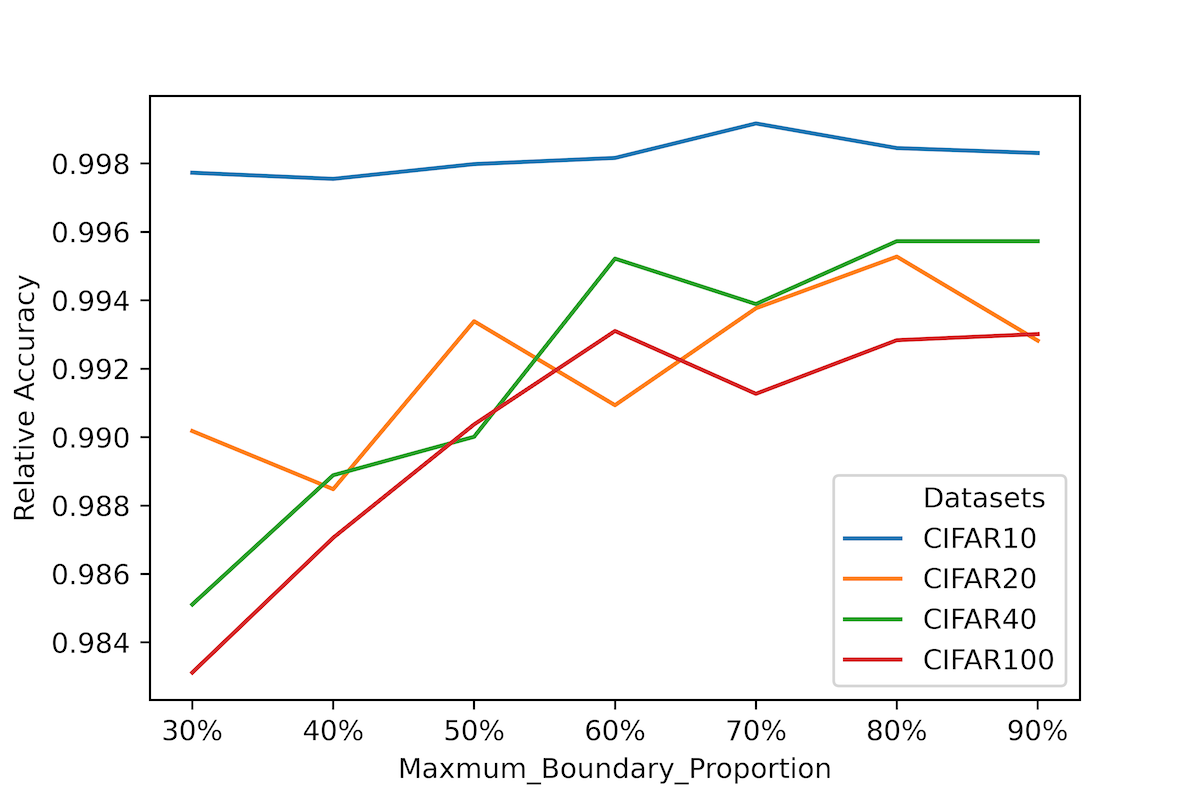
\includegraphics[width=0.8\textwidth]{src/bwcl_relative_size04.png}
 \caption{The BWCL test set accuracies. Averaged with 3 individual runs. The threshold is 10\%. Horizontal axis is the percentage of samples selected, in term of EDGIS selected samples. Vertical axis is the accuracy score.}
 \label{Fig.logistic_subsets}
 \end{figure}

\section{Experiment 4: Data Reduction for CNN}
\label{CNN}
We train the network densenet101, three times, with learning rate 0.1 (150 epochs), 0.01 (100 epochs) and 0.001 (100 epochs)

\begin{table}[H]
    \centering
    \begin{tabular}{|l|l|l|l|l|l|l|}
    \hline
        Datasets & Retention Rate  & POP & EGDIS & CL & WCL & BWCL \\ \hline
        CIFAR10 & 14.915\% & 86.80\% & 85.18\% & 86.71\% &\textbf{88.36}\% & 86.75\% \\ \hline
        CIFAR20 & 16.67\% & 59.93\% & 61.43\% & \textbf{70.96}\% & 69.34\% & 64.67\% \\ \hline
        CIFAR40 & 21.09\% & 63.99\% & 63.89\% & \textbf{75.77}\% & 71.36\% & 70.65\% \\ \hline
        CIFAR100 & 31.48\% & 75.24\% & 73.74\% & 82.72\% & \textbf{83.23}\% & 81.69\% \\ \hline
    \end{tabular}
    \caption{CNN test set relative accuracy}
    \label{132e3213}
\end{table}

\begin{figure}[H]
\centering  
\subfigure[Relative Accuracy]{
\label{Fig.sub.a1}
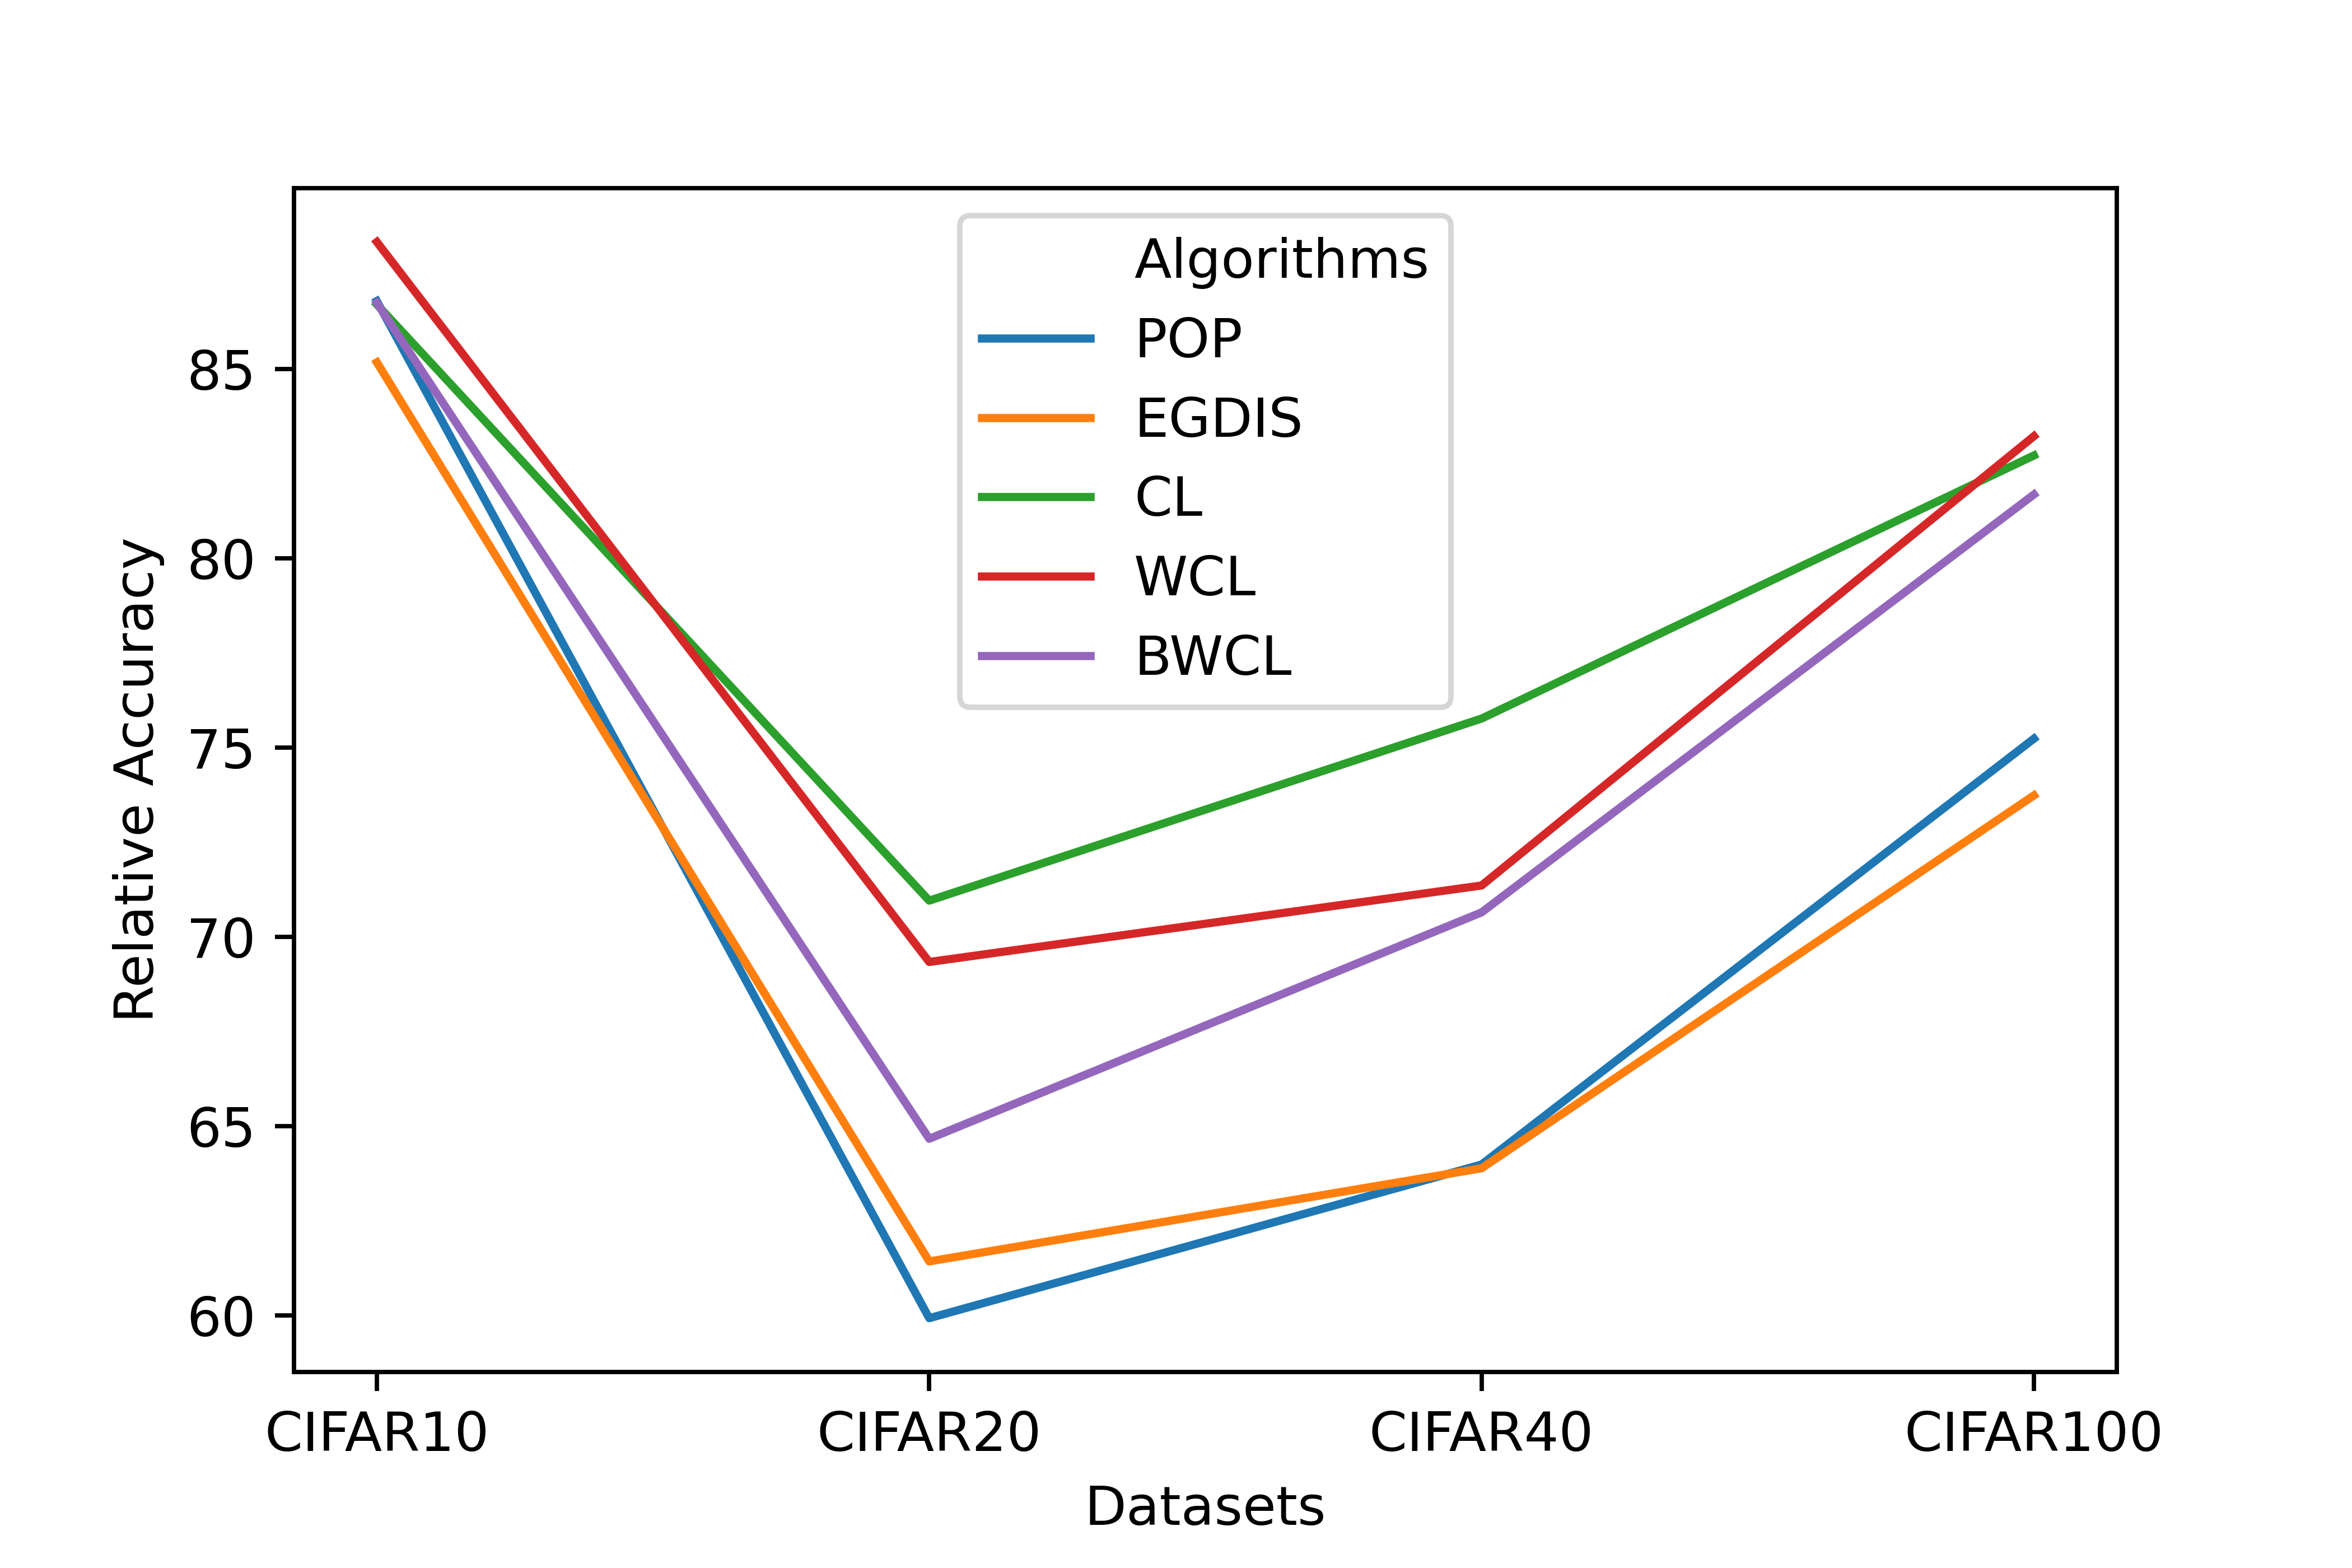
\includegraphics[width=0.45\textwidth]{src/cnn-alg-relative.png}}
\subfigure[Relative Accuracy of BWCL by tuning maximum boundary proportion]{
\label{Fig.sub.a2}
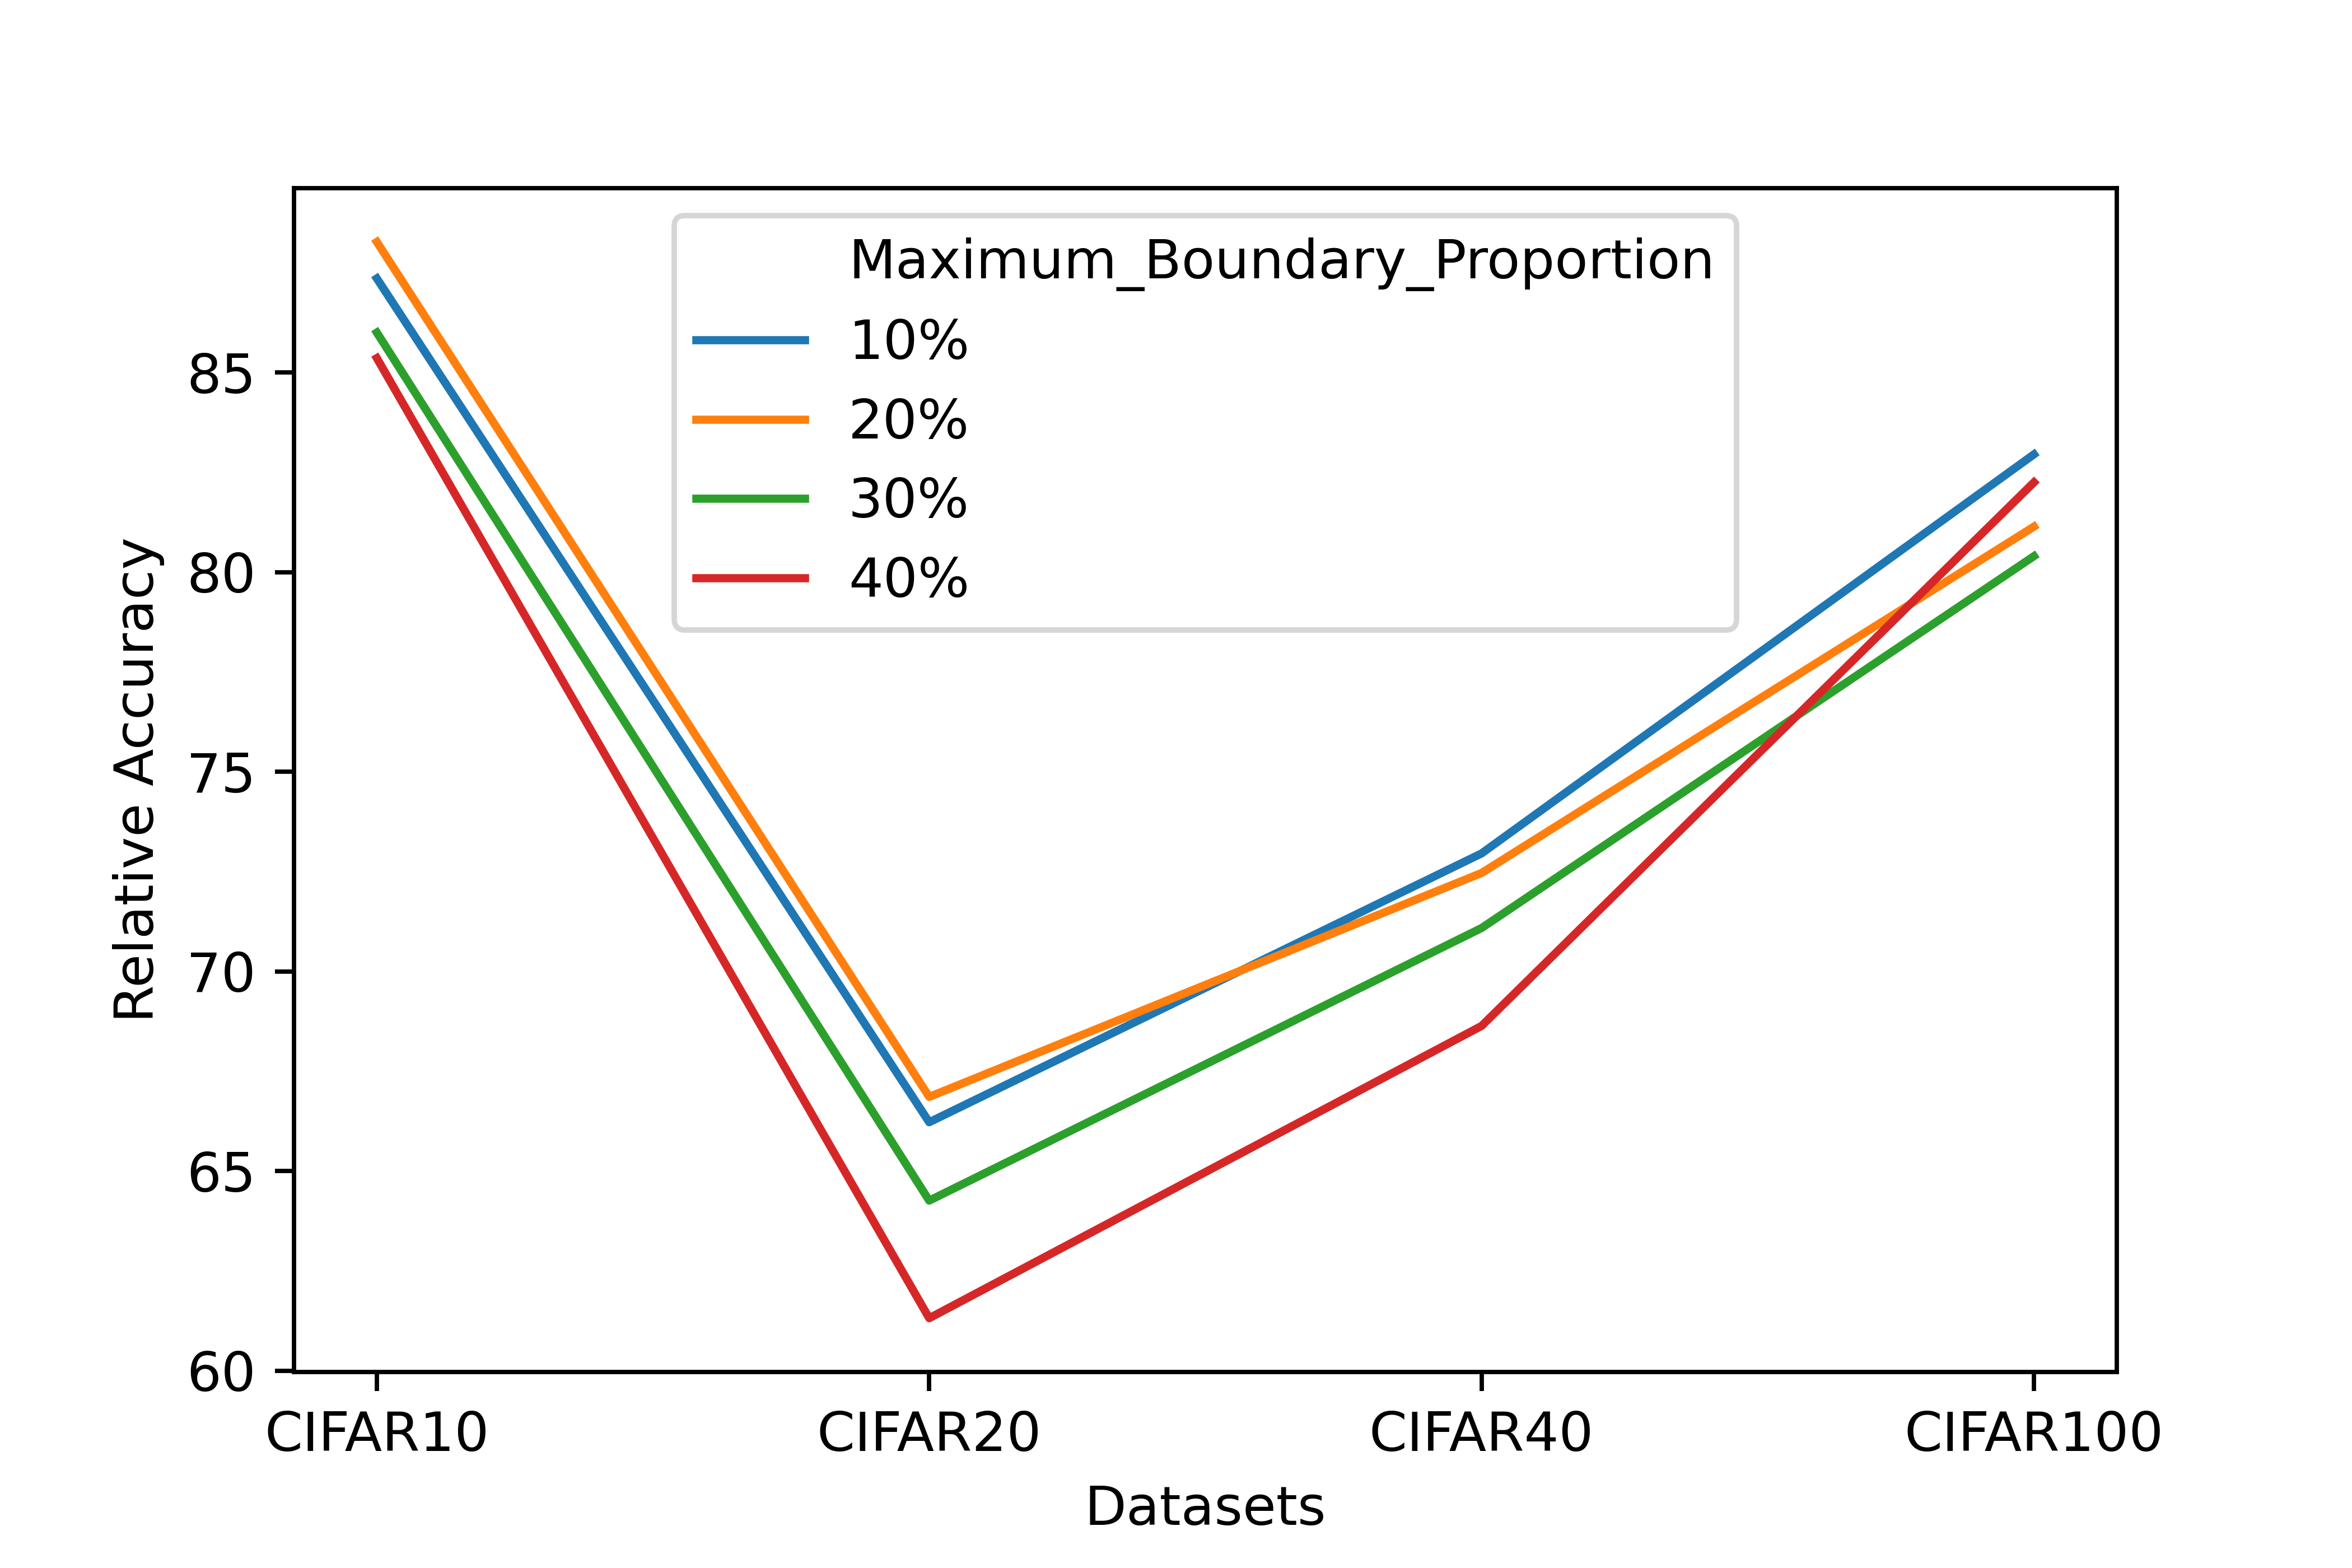
\includegraphics[width=0.45\textwidth]{src/cnn-bwcl-relative.png}}
\caption{Relative Accuracy of data reduction algorithms}
\label{Fig.logistic_relativeacc}
\end{figure}


\begin{figure}[H]
\centering  
\subfigure[CIFAR10]{
\label{Fig.sub.a1}
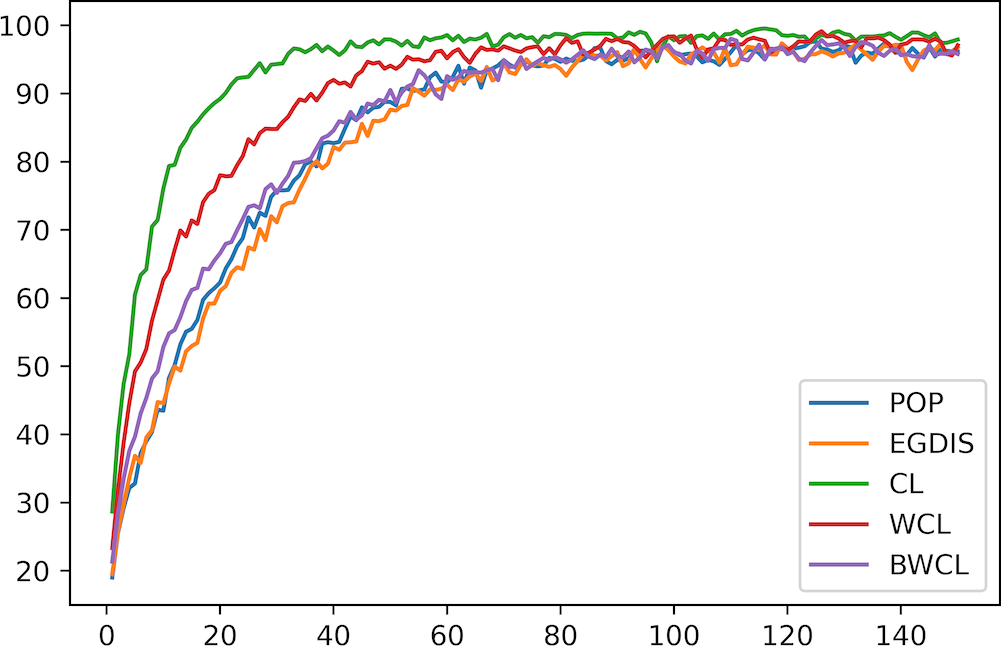
\includegraphics[width=0.45\textwidth]{src/trend_cifar10.png}}
\subfigure[CIFAR100]{
\label{Fig.sub.a2}
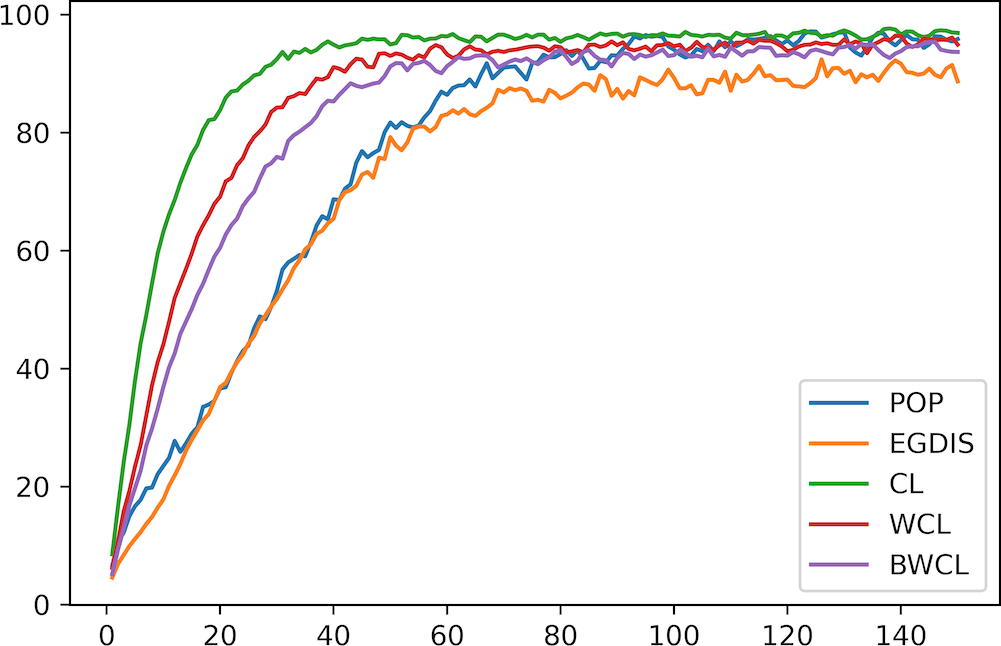
\includegraphics[width=0.45\textwidth]{src/trend_cifar100.png}}

\subfigure[CIFAR20]{
\label{Fig.sub.a2}
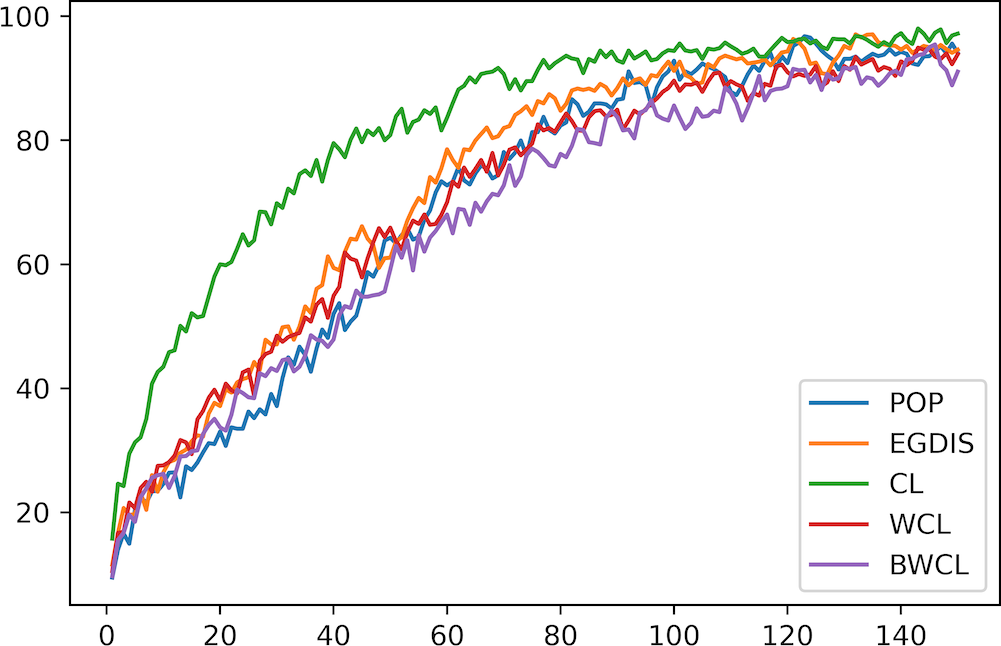
\includegraphics[width=0.45\textwidth]{src/trend_cifar20.png}}
\subfigure[CIFAR40]{
\label{Fig.sub.a2}
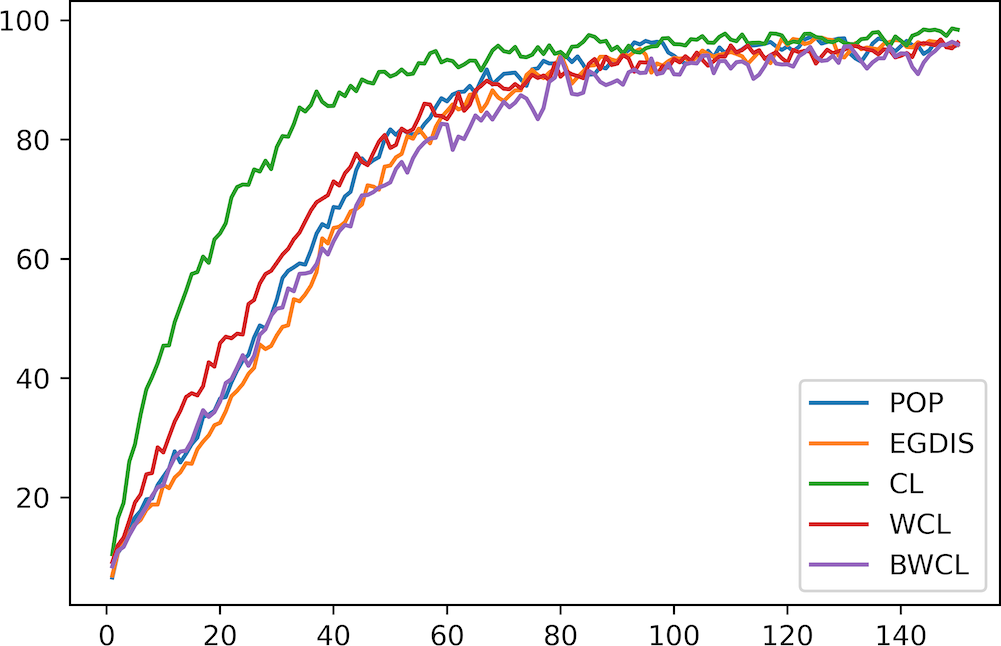
\includegraphics[width=0.45\textwidth]{src/trend_cifar40.png}}
\caption{The training trend of four datasets by selecting the same amount of samples as EGDIS, of the first 150 epochs}
\label{Fig.training_trend}
\end{figure}
